% Format teze zasnovan je na paketu memoir
% http://tug.ctan.org/macros/latex/contrib/memoir/memman.pdf ili
% http://texdoc.net/texmf-dist/doc/latex/memoir/memman.pdf
% 
% Prilikom zadavanja klase memoir, navedenim opcijama se podešava 
% veličina slova (12pt) i jednostrano štampanje (oneside).
% Ove parametre možete menjati samo ako pravite nezvanične verzije
% mastera za privatnu upotrebu (na primer, u b5 varijanti ima smisla 
% smanjiti 
\documentclass[12pt,oneside]{memoir}
\sloppy
\usepackage{cmap}

% Paket koji definiše sve specifičnosti mastera Matematičkog fakulteta
\usepackage{matfmaster}
\usepackage{hyperref}
\hypersetup{colorlinks,linkcolor={blue},citecolor={blue},urlcolor={blue}}

%\usepackage[T1]{fontenc}
\usepackage{xcolor}
\usepackage{listings}

\lstset{
language=Scala,
basicstyle=\small\ttfamily,
columns=fullflexible,
keywords=[2]{fail},
keywords=[3]{pass},
keywordstyle={\color{blue!80!black}},
keywordstyle=[2]{\color{red!80!black}},
keywordstyle=[3]{\color{green!50!black}},
showstringspaces=false
}
%
% Podrazumevano pismo je ćirilica.
%   Ako koristite pdflatex, a ne xetex, sav latinički tekst na srpskom jeziku
%   treba biti okružen sa \lat{...} ili \begin{latinica}...\end{latinica}.
%
% Opicija [latinica]:
%   ako želite da pišete latiniciom, dodajte opciju "latinica" tj.
%   prethodni paket uključite pomoću: \usepackage[latinica]{matfmaster}.
%   Ako koristite pdflatex, a ne xetex, sav ćirilički tekst treba biti
%   okružen sa \cir{...} ili \begin{cirilica}...\end{cirilica}.
%
% Opcija [biblatex]:
%   ako želite da koristite reference na više jezika i umesto paketa
%   bibtex da koristite BibLaTeX/Biber, dodajte opciju "biblatex" tj.
%   prethodni paket uključite pomoću: \usepackage[biblatex]{matfmaster}
%
% Opcija [b5paper]:
%   ako želite da napravite verziju teze u manjem (b5) formatu, navedite
%   opciju "b5paper", tj. prethodni paket uključite pomoću: 
%   \usepackage[b5paper]{matfmaster}. Tada ima smisla razmisliti o promeni
%   veličine slova (izmenom opcije 12pt na 11pt u \documentclass{memoir}).
%
% Naravno, opcije je moguće kombinovati.
% Npr. \usepackage[b5paper,biblatex]{matfmaster}

% Pomoćni paket koji generiše nasumičan tekst u kojem se javljaju sva slova
% azbuke (nema potrebe koristiti ovo u pravim disertacijama)
\usepackage{pangrami}
\usepackage[utf8]{inputenc}
\usepackage[english, serbian]{babel}
\usepackage{amsthm}
\usepackage{graphicx}
%\usepackage{caption}
\usepackage{subfig}
%\usepackage{subfigure}
\setcounter{tocdepth}{3}
\setsecnumdepth{subsubsection}

% Datoteka sa literaturom u BibTex tj. BibLaTeX/Biber formatu
\bib{tezaBib}

% Ime kandidata na srpskom jeziku (u odabranom pismu)
\autor{Aна Д. Митровић}
% Naslov teze na srpskom jeziku (u odabranom pismu)
\naslov{Примена Скале у паралелизацији расплинутог тестирања}
% Godina u kojoj je teza predana komisiji
\godina{2018}
% Ime i afilijacija mentora (u odabranom pismu)
\mentor{др Милена Вујошевић Јаничић, доцент\\ Универзитет у Београду, Математички факултет}
% Ime i afilijacija prvog člana komisije (u odabranom pismu)
\komisijaA{др Саша Малков, ванредни професор\\ Универзитет у Београду, Математички факултет}
% Ime i afilijacija drugog člana komisije (u odabranom pismu)
\komisijaB{др Александар Картељ, доцент\\ Универзитет у Београду, Математички факултет}
% Ime i afilijacija trećeg člana komisije (opciono)
% \komisijaC{}
% Ime i afilijacija četvrtog člana komisije (opciono)
% \komisijaD{}
% Datum odbrane (obrisati ili iskomentarisati narednu liniju ako datum odbrane nije poznat)
\datumodbrane{15. јануар 2016.}

% Apstrakt na srpskom jeziku (u odabranom pismu)
\apstr{%
}

% Ključne reči na srpskom jeziku (u odabranom pismu)
\kljucnereci{}

\begin{document}
% ==============================================================================
% Uvodni deo teze
\frontmatter
% ==============================================================================
% Naslovna strana
\naslovna
% Strana sa podacima o mentoru i članovima komisije
\komisija
% Strana sa podacima o disertaciji na srpskom jeziku
\apstrakt
% Sadržaj teze
\tableofcontents*

% ==============================================================================
% Glavni deo teze
\mainmatter
% ==============================================================================

% ------------------------------------------------------------------------------
\chapter{Увод}
% ------------------------------------------------------------------------------

% ------------------------------------------------------------------------------
\chapter{Програмски језик Скала}
\label{chp:razrada}
% ------------------------------------------------------------------------------

Скала је језик опште намене настао 2003. године са циљем да превазиђе ограничења програмског језика Јава комбиновањем објектно оријентисанe и функционалнe програмске парадигме. Мотивација иза овакве идеје је не ограничавати се на једну од ових парадигми и њених предности већ искористити најбоље из оба света. Управо због овакве комбинације парадигми Скала је веома погодна за решавање различитих врста проблема, почевши од малих незахтевних скриптова па све до великих компликованих система. На основу ове прилагодљивости је и добила своје име: реч "скала" означава "скалабилан језик" (енг. \textit{scalable language}), односно језик који ће се прилагођавати и расти заједно са потребама система \cite{progInScala}.
\par Творац Скале је Мартин Одерски (нем. \textit{Martin Odersky}) (1958-), немачки научник и професор на универзитету EPFL (École Polytechnique Fédérale de Lausanne) у Лозани, Швајцарској. Још док је био студент, имао је жељу да напише језик који ће подржавати објектну и функционалну парадигму, говорећи да су ове две парадигме само две стране истог новчића. Желео је да се тај језик преводи у Јава бајт к\^{о}д али и да превазиђе ограничења језика Јава. Први резултат оваквог његовог рада је био језик Funnel, који због свог минималистичког дизајна није заживео. Затим је настала Скала, коју је професор Одерски	 развијао од 2001. године заједно са својом групом на универзитету EPFL. Познат је и по другим радовима, као што je имплементација GJ (Generic Java) компајлера који је постао основа javac компајлера \cite{MartinEpfl, ScalaHistory}.

\section{Опште карактеристике}

Ово су неке од најважнијих особина Скале \cite{progInScala}:

\begin{description}
\item \textbf{Компатибилност са Јавом} Скала није сама по себи продужење Јаве али је потпуно компатибилна са њом: њен изворни к\^{о}д се преводи у Јава бајт к\^{о}д који се извршава на Јава виртуелној машини. Из кода писаног у Скали је омогућено коришћење Јава библиотека, класа, интерфејса, метода, поља и типова. Омогућено је и обрнуто, позивање Скала кода из Јаве, мада се оно ређе користи. Такође, Скала омогућава лакшу и лепшу употребу Јава типова уз помоћ имплицитне конверзије омогућавајући употребу својих метода за манипулацију типовима. Компатибилност олакшава програмерима лакши прелазак из Јаве у Скалу јер нису принуђени да се одједном одрекну написаног кода у Јави.

Корен Скале није само језик Јава, иако је Јава имала највећи утицај у њеном стварању. Идеје и концепти из разних језика, како објектно оријентисаних тако и функционално оријентисаних, су инспирисали развој Скале. Међу њима су језици: C\#  од кога је Скала преузела синтаксне конвенције, Erlang чије идеје су сличне идејама конкурентности базиране на моделу Actors и други: C, C++,  Smalltalk, Ruby, Haskell, SML, F\# итд.

\item \textbf{Објектно оријентисана парадигма} Писање програма и смештање података и њихових својстава у класе и објекте тих класа је веома популарно и интуитивно програмерима. Скала је то задржала притом мало изменивши концепт. У многим језицима, укључујући и Јаву, дозвољене су вредности  које нису објекти или које нису у склопу објекта. То могу бити примитивне вредности у Јави или статичка поља и методи. Скала то не дозвољава и зато је објектно оријентисан језик у \textit{чистој форми}: "Свака вредност је објекат и свака операција је позив метода" \cite{progInScala}. Елегантан начин коришћења метода налик на операције је један од начина на који се Скала брине да програмерима буде пријатно њено коришћење.

\item \textbf{Концизност} Скала к\^{о}д има тенденцију да буде краћи од Јава кода, чак се процењује да има барем два пута мање линија кода од Јаве. Постоје и екстремни случајеви где је број линија и десет пута мањи. Ова особина није значајна само због тога што знатно олакшава програмирање, већ олакшава читање кода и откривање грешака којих ионако има мање јер има мање простора за њих. Ово је нешто што одликује саму синтаксу језика, а веома помажу и разне библиотеке које имају већ имплементиране многе функције које врше послове са којима се често сусрећемо. Лако се и имплементирају и касније употребљавају библиотеке које сами напишемо. Такође, Скала подржава аутоматско закључивање типова (енг. \textit{type inference}) што омогућава изостављање понављања већ наведених типова, што резултује читљивијим кодом.

\item \textbf{Висок ниво} Како је Скала погодна и за велике и комплексне системе она се труди да се прилагоди њиховим захтевима подижући ниво апстракције у свом коду. Омогућава много једноставнији и краћи начин кодирања разних проблема. Рецимо, уместо да пролазимо кроз ниску карактера карактер по карактер користећи петљу, у Скали се то може урадити у једној линији кода помоћу \textit{предиката} тј.  \textit{функцијских литерала} који су детаљније објашњени у поглављу \ref{sec:funkDeoJezika}. Скала к\^{о}д тежи да буде разумљивији и мање комплексан како би олакшао већ комплексан систем који се имплеметира.

\item \textbf{Статичка типизираност} Скала је статички типизиран језик што значи да се типови података који су коришћени знају у време компилације. Неки сматрају ово маном као и да је навођење типова сувишно поред техника тестирања софтвера као што је нпр. тестирање јединица кода (енг. \textit{unit testing}). Ипак, у Скали је статичка типизираност напреднија јер нам дозвољава да изоставимо тип на местима где би он био поновљен и вероватно би нам само сметао. Због оваквих понављања која су неопходна у неким језицима, многи се одрекну предности статички типизираних језика као што су: детектовање разних грешака у време компилације, лакше рефакторисање кода и коришћење типова као вид документације.

\item \textbf{Својствa} Скала уводи појам својстава (енг. \textit{trait}) који делe карактеристике са интерфејсима и наслеђивањем класа у Јави. У својствима као и у интерфејсима можемо декларисати методе, али и дефинисати поља и конкретне методе што није могуће у интерфејсима. Променљиве омогућавају чување стања а методе дефинисање одређеног понашања. То чини својства богатијим од интерфејса.  Кажемо да се својства "миксују" у класе (енг. \textit{mix in}). У једну класу је могуће миксовати више својстава.

Миксовање се може остварити кључном речју \textbf{extends} и у том случају класа наслеђује суперкласу својства. У случају да желимо да класа наследи неку другу класу, онда помоћу \textbf{extends} дефинишемо суперкласу а својства миксујемо помоћу \textbf{with} као што је илустровано у наредном примеру \cite{progInScala}: 

\begin{lstlisting}[language=Scala]
class Animal
trait HasLegs
trait Philosophical
/* Superklasa "Animal" i miksovana svojstva "HasLegs" i "Philosophical" */
class Frog extends Animal with HasLegs with Philosophical {
	/* ... */
}
\end{lstlisting}

Највећа разлика између класе и својства односи се на позивање метода надкласе помоћу поља \textit{super}. На пример, позивом метода \textit{super.toString()} у случају класе, тачно се зна који ће метод \textit{toString()} бити позван јер се зна надкласа дате класе. У случају својства, не можемо знати на шта се овај позив односи јер то директно зависи од класе у коју ће дато својство бити миксовано, као и од претходно миксованих својстава. То значи да се \textit{super} позиви одређују \textit{динамички}. Свако миксовано својство може позвати метод претходно миксованог својства. Ово омогућава класама да постигну различито понашање у зависности од редоследа миксованих својстава. Помоћу малог броја дефинисаних својстава може се постићи много различитих циљева комбиновањем редоследа миксовања.

\end{description}
\par Карактеристика која највише раздваја Скалу од Јаве је њена \textbf{функционалност} - Скала у потпуности подржава функционално програмирање. Ова особина је детаљно објашњена у следећем поглављу.

% --------
\section{Функционални део језика}
\label{sec:funkDeoJezika}

Функцинална парадигма се развија од 1960-тих година. У њеној основи леже \textit{ламбда рачун} (енг. \textit{$\lambda$-calculus}) и комбинаторна логика. Ламбда рачун представља математичку апстракцију и формализам за описивање функција и њихово израчунавање. Њега је увео Алонзо Черч (енг. \textit{Alonzo Church}) 1930-тих година а Алан Тјуринг (енг. \textit{Alan Turing}) је 1937. године показао да је експресивност ламбда рачуна еквивалентна експресивности Тјурингових машина. Иако је ламбда рачун првобитно развијен само за потребе математике, данас се он сматра првим функционалним језиком. Други модел рачунања који је утицао на функционалне програмске језике, комбинаторну логику, створили су Мојсеј Шејнфинкел (рус. \textit{Моисей Шейнфинкель}) и Хаскел Кари (енг. \textit{Haskell Curry}) 1924. године са циљем да елиминишу употребу променљивих у математичкој логици \cite{funkMilena, history, lambdaRacun, history}.
\par Најстарији виши функционални програмски језик је LISP који је пројектовао Џон Макарти (енг. \textit{John McCarthy}) на институту МИТ (Масачусетски технолошки институт) 1958. године. Након тога се полако развијају и други функционални језици као што су ISWIM, FP, Scheme, ML, Miranda, Erlang, SML, Haskell, OCAML,  F\#, Elixir итд. Поред функционалних језика постоје и језици који нису функционални али  у одређеној мери подржавају функционалне концепте или могу да их остваре на други начин, нпр. Java, C, C$++$, C\#, Phyton  \cite{funkMilena, history}.
\par Разлика између императивне и функционалне парадигме се може описати дефинисањем самог програма \cite{funkMalkov}:
\begin{itemize}
\item Императивна парадигма: 
\\Програм представља формално упутство о томе шта рачунар треба да ради да би урадио неки посао
\\Програм представља одговор на питање КАКО се нешто РАДИ
\item Функционална парадигма:
\\Програм представља формално објашњење онога што рачунар треба да израчуна
\\Програм представља одговор на питање ШТА се РАЧУНА
\end{itemize}
\par Функционални језици су веома блиски математици због чега се и називају \textit{функционалним} језицима: њихове функције се понашају као функције у математичком смислу. О томе говоре следећа два концепта којима се воде функционални језици \cite{progInScala}: 
\\
\par Први концепт се односи на \textbf{"статус" функција}. У функционалним језицима функције су вредности \textit{првог реда}, тј. \textit{грађани првог реда}. То значи да се оне могу користити као вредности типова као што су нпр. цели, реални бројеви, ниске карактера итд. Статус оваквих типова се не разликује од статуса функција, што у многим језицима није случај. Ово омогућава коришћење функција на природан, концизан и читљив начин: као аргументе других функција, повратне вредности функција, њихово чување у променљивим, угњеждавање и слично. Другим речима, функције се креирају и прослеђују без икаквих рестрикција на које смо навикли у императивним језицима.
\par У Скали можемо користити локалне (угњеждене) функције које су често веома мале и лако се комбинују како би заједно заокружиле један већи посао. Ово одговара функционалном стилу који промовише следећу идеју: програм треба изделити на много мањих функција (целина) од којих свака има јасно дефинисан задатак.
\par Посебно су корисни и важни \textit{функцијски литерали} који представљају функције које могу бити неименоване (анонимне функције) и прослеђиване као обичне вредности. Назив "функцијски литерал" се користи за функције у изворном коду, а у време извршавања оне се називају \textit{"функцијским вредностима"} (разлика слична разлици између класа и објеката у објектно оријентисаним језицима). Функцијске вредности су објекти које можемо чувати у променљивама али су истовремено и функције које можемо позивати. Пример функцијског литерала који инкрементира цео број изгледа овако \cite{progInScala}:
\begin{lstlisting}[language=Scala]
var increase = (x: Int) => x + 1
increase(10)
\end{lstlisting}
Променљива \textbf{increase} је објекат који садржи литерал, али је и функција коју позивамо са аргументом 10.
\\
\par Други концепт се односи на \textbf{непостојање стања} које се иначе представља променљивама у програму. То значи да извршавање метода нема\textit{ "бочне ефекте"}, односно да функције које позивамо не мењају податке "у месту" већ враћају нове вредности као резултате свог израчунавања. Избегава се (у чисто функционалним језицима се избацује) кад год је то могуће коришћење променљивих које мењају своје стање, а за промену се користе променљиве код којих то није дозвољено. То су променљиве које се иницијализују само једном. Оне се у Скали дефинишу помоћу кључне речи \textbf{val} и покушај промене вредности ове променљиве након што је иницијализована резултирао би грешком. Променљиве које су стандардне у императивним језицима и које можемо мењати по потреби се дефинишу кључном речју \textbf{var}.
\par Непостојање стања има за последицу избацивање итеративних конструкција. Овакав резон може испрва деловати чудно, међутим све што се може остварити кроз итерације се може остварити и \textit{рекурзијом}. Рекурзија је у функционалним језицима потпуно природна и неизбежна. Некада се решења проблема који захтевају стање у оваквим језицима превише закомпликују, али оно се може направити по потреби на друге начине тако да се ово не сматра недостатком. Предност је у томе што не морамо пратити вредности променљивих и њихове промене што олакшава разумевање програма. Један програм у функционалном језику представља низ дефиниција и позива функција а његово извршавање је евалуација тих функција \cite{funkMilena}.
\par Као пример метода који нема бочне ефекте може послужити метод \textbf{replace} који као аргументе добија ниску карактера и два карактера. Његов задатак је да у датој ниски замени сва појављивања једног карактера другим карактером. Он неће променити ниску коју је добио као аргумент, већ ће вратити нову која више нема појављивања датог карактера који смо заменили новим.  
\par Ова особина метода без бочних ефеката назива се \textit{референтна прозирност} (енг. \textit{referential transparency}): "за било које вредности аргумената позив метода се може заменити својим резултатом без промене семантике програма" \cite{progInScala}. Пример:

\begin{lstlisting}[language=Scala]
val p = previous(90)
\end{lstlisting}
Свако појављивање променљиве \textbf{p} можемо заменити изразом \textbf{previous(90)}.

Позив метода можемо заменити његовим резултатом јер смо сигурни да ће при сваком позиву са истим вредностима аргумената вратити исти резултат. Вредност резултата не зависи од бочних ефеката и тренутног стања променљивих, већ само од вредности прослеђених аргумената. Због тога, редослед позива таквих метода није важан и може бити произвољан. За овакве методе кажемо да су референтно прозирни или транспарентни. Они су концизнији, читљивији и производе мање грешака јер немају пропратне ефекте. Ипак, у пракси су нам углавном неопходни пропратни ефекти због чега они могу бити присутни на контролисан начин. У том случају, програмски језик више није чисто функционалан \cite{funkMilena}. 
\\
\par Чисто функционални језици (нпр. Haskel, Miranda) захтевају коришћење имутабилних структура података,  референтно прозирних метода и рекурзије. Други језици, као што су Скала, Python, Ruby итд. охрабрују овакво програмирање али не условљавају програмера. Скала омогућава бирање начина за решавање проблема и нуди функционалне алтернативе за све императивне конструкције. На овај начин програмер се полако и без притиска навикава на другачији начин размишљања \cite{funkMilena, progInScala}.
\par Неке од карактеристика које Скала подржава а које су заједничке и другим функционалним језицима су \cite{progInScala}:
\begin{description}
	\item \textbf{Функције вишег реда} %strana 210
Функције вишег реда су оне које имају друге функције као своје аргументе. Оне поједностављују к\^{о}д и смањују његово понављање. Ово је пример функције која као аргументе има ниску карактера \textbf{query} и другу функцију \textbf{matcher}:
\begin{lstlisting}[language=Scala]
def filesMatching(query: String, 
		matcher: (String, String) => Boolean) = {
	for (file <- filesHere; if matcher(file.getName, query))
		yield file
}
\end{lstlisting}
Функција \textbf{filesMatching} треба да међу датотекама \textbf{filesHere} пронађе датотеке које испуњавају неки критеријум. Да се к\^{о}д не би понављао за сваки критеријум појединачно, он се прослеђује функцији као аргумент у виду функције \textbf{matcher}. Сам критеријум представља функцију која има две ниске карактера као аргумент, и враћа логички тип - тачно ако је критеријум испуњен и нетачно у супротном.
\par Следећи пример демонстрира коришћење функције вишег реда из Скала библиотеке:
\begin{lstlisting}[language=Scala]
def containsOdd(nums: List[Int]) = nums.exists(_ % 2 == 1)
\end{lstlisting}
Метод \textbf{exists} проверава постојање елемента листе \textbf{nums} који задовољава наведени предикат који му је прослеђен као аргумент (дељивост са 2).  Постоји доста метода сличних методу exists, попут: \textbf{find}, \textbf{filter}, \textbf{foreach}, \textbf{forall}, итд.

\item \textbf{Каријеве функције} %strana 214
Каријеве функције уместо једне листе аргумената узимају аргументе један по један, имајући више листи које садрже по један аргумент. На овај начин омогућују дефинисање функција помоћу већ дефинисаних на следећи начин:
\begin{lstlisting}[language=Scala]
def curriedSum(x: Int)(y: Int) = x + y
\end{lstlisting}
Ово је функција која сабира два цела броја. Када је позовемо на овај начин:
\begin{lstlisting}[language=Scala]
curriedSum(1)(2)
\end{lstlisting}
десиће се два позива функције. Први позив ће узети први параметар \textbf{x} и вратити другу функцију која узима параметар \textbf{y}, и враћа збир ова два параметра. Прва и друга функција би редом изгледале овако:
\begin{lstlisting}[language=Scala]
def first(x: Int) = (y: Int) => x + y
val second = first(1) /* poziv prve funkcije */
second(2) /* poziv druge funkcije */
\end{lstlisting}
Каријев поступак има пуно примена. Рецимо, можемо дефинисати функцију која додаје број 1 неком целом броју:
\begin{lstlisting}[language=Scala]
val onePlus = curriedSum(1)_
onePlus(2) /* --> vraca 3 */
\end{lstlisting}
Позивамо Каријеву функцију \textbf{curriedSum} користећи \textbf{$\_$} као знак да на том месту може бити било која вредност (енг. \textit{wildcard}). Суштина је да је функција \textbf{onePlus} дефинисана помоћу Каријеве функције која сабира било која два цела броја, а код које је први аргумент везан за број 1.
\item \textbf{Упаривање образаца}
\label{uparObr}
Честo је потребно препознати да ли неки израз има одређену форму тј. да ли одговара одређеном обрасцу. То је корисно уколико треба да се имплементира функција која ради различите ствари у зависности од типова аргумената. Уобичајени примери су аритметичке операције или секвенце одређеног типа. Ово је пример са листама: 
\begin{lstlisting}[language=Scala]
expr match {
	case List(0, _, _) => println("found it")
	case _ =>
}
\end{lstlisting}
Помоћу кључне речи \textbf{match} проверавамо да ли израз \textbf{expr} одговара некој листи од три елемента којој је први елемент 0 а друга два било који бројеви. Пошто се израз \textbf{expr} пореди редом са случајевима како су наведени, након неуспешног поређења са трочланом листом успешно ће се упарити са \textbf{$\_$} који служи као образац који одговара свему (енг. \textit{wildcard pattern}). 

\item \textbf{Comprehensions}
Конструкција \textbf{for expression} или \textbf{for comprehension} се често користи у Скали не само за стандардно итерирање кроз колекције већ и на другачије начине, на пример:
\begin{lstlisting}[language=Scala]
val forLineLengths =
	for {
		file <- filesHere 	/* iteriranje kroz listu fajlova */
		if file.getName.endsWith(".scala") 	/* prvi uslov */
		line <- fileLines(file) 	/* iteriranje kroz linije fajla */
		trimmed = line.trim 	/* dodela promenljivoj trimmed */
		if trimmed.matches(".*for.*") 	/* drugi uslov */
	} yield trimmed.length 		/* povratna vrednost */
\end{lstlisting}
Овај пример обухвата пуно могућности које пружају \textbf{for} изрази. Прво, итерирање кроз листу \textbf{filesHere} користећи \textbf{<-} метод. Друго, филтрирање тих датотека помоћу услова задатог у \textbf{if} изразy. Онда следи једна угњеждена петља где се врши итерација кроз линије тренутног фајла (који је испунио услов, а ако није, прелази се на следећи фајл). Након тога, чување тренутне линије без вишка бланко карактера у променљивој \textbf{trimmed} и још један \textbf{if} израз. Најзад, помоћу \textbf{yield} наредбе враћа се дужина линије чиме се попуњава листа \textbf{forLineLengths}. Дакле, можемо користити угњеждене петље, филтрирати резултате, чувати податке у променљивама и попуњавати колекције помоћу \textbf{yield} наредбе. Све ове опције нам омогућавају конструкције које подсећају на дефинисање елемената скупова у математици.
\end{description}

\par Управо функционална својства Скале су кључни разлози због којих је она веома погодна за паралелизацију израчунавања. 
%--------

% --------
\section{Паралелизам}
Потреба за све већом моћи процесора непрекидно расте у складу са захтевнијим апликацијама. "Направи десет пута бржи процесор, и софтвер ће убрзо наћи десет пута више посла" \cite{freeLunch}. Другим речима, стандарди расту докле год расту и могућности. Потребно је све брже и ефикасније извршавати захтевна израчунавања. Зато су годинама откривани и развијани разни начини побољшања перформанси процесора као што су повећавање брзине откуцаја часовника, оптимизација тока извршавања и повећавање простора кеш меморије на чипу. Ова побољшања се односе и на секвенцијалне, непаралелне апликације као и на конкурентне апликације. Ипак, ови начини подизања перформанси полако достижу свој максимум. Муров закон каже да се број транзистора на процесорском језгру дуплира на сваких осамнаест месеци, описујући експоненцијалан раст броја транзистора. Као и друге области које експоненцијално напредују, ни ова не може напредовати вечно и у једном тренутку раст више неће бити могућ. Поставља се питање шта ће бити када достигнемо ограничења свих побољшања на која смо навикли? Још увек има простора за раст, али јавила се потреба за новим идејама. Тако је напредак процесора почео све више да се односи на број \textit{централних процесорских јединица} тј. \textit{језгара}. Данас имамо \textit{multi-core} процесоре који имају у просеку од 2 до 8 процесорских језгара, и \textit{many-core} процесоре са стотинама, па и хиљадама језгара. Сматра се да је конкурентност нова главна револуција у писању софтвера \cite{freeLunch, survey}.

Како главне улоге у новим побољшањима имају конкуретност и паралелизација, следе њихове дефиниције и појашњења \cite{survey, konkMalkov, progInScala3}:  
%\theoremstyle{definition}
\newtheorem{definition}{Дефиниција}
\begin{definition}
\textit{За два процеса кажемо да се извршаваjу \textbf{конкурентно} ако ниjе унапред позната њихова међусобна временска лоцираност.}
\end{definition}
Ово значи да имамо два процеса којима ће распоређивач (енг. \textit{scheduler}), као нпр. Јава виртуелна машина, наизменично да додељује "кришке" времена (енг. \textit{time-slice}). Због овога имамо привид да се ова два процеса извршавају дословно истовремено иако то није случај. Конкурентно извршавање се обично одвија када процеси деле једну процесорску јединицу.
%Може се рећи следеће: "Конкурентност је начин на који излазимо на крај са много послова истовремено."
%"Паралелизам је начин на који извршавамо више послова истовремено."
\begin{definition}
\textit{Два процеса се извршаваjу \textbf{паралелно} ако постоjи период времена у коме су оба процеса истовремено активнa.}
\end{definition}

У случају паралелног израчунавања процеси се извршавају дословно истовремено на различитим процесорским јединицама.
Паралелно израчунавање је подскуп конкурентног израчунавања, тј. може се представити као још један од начина на који се постиже конкурентност. Можемо написати конкурентну апликацију која има више просеца или нити, а са додатним језгрима процесора она може постати и паралелна. 

Људи често мешају конкурентност и паралелизам и користе их као синониме, иако постоји разлика између њих. Ове појмове не треба тек тако мешати. Њихова различитост је демонстрирана сликама \ref{fig:ParVSCon1} и \ref{fig:ParVSCon2}.
\begin{figure}[!ht]
  \centering
  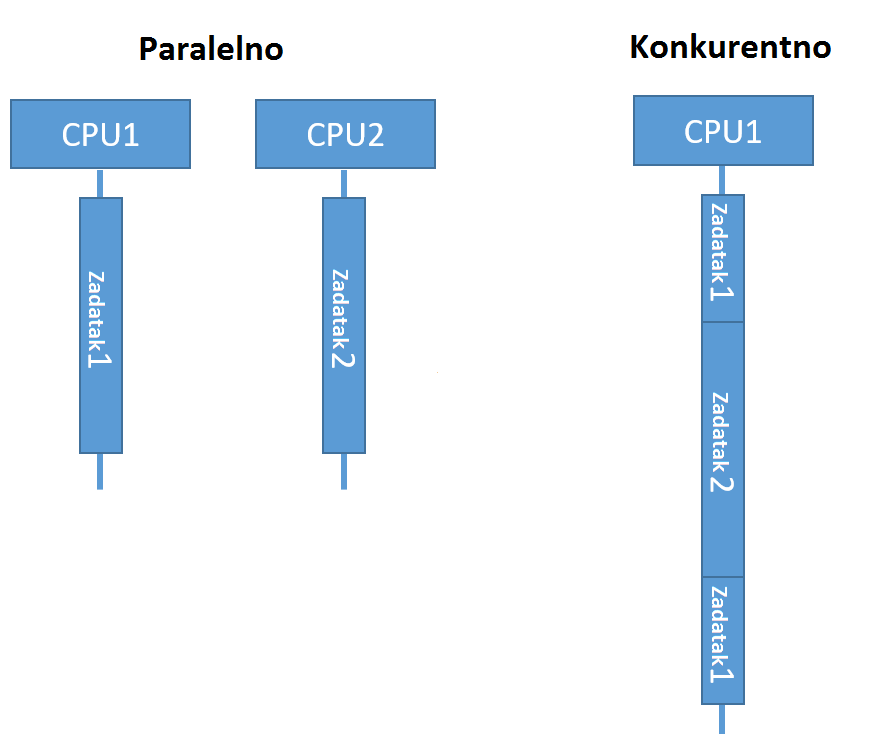
\includegraphics[width=0.6\textwidth]{parallel-vs-concurrent-dotnet-core.png}
  \caption{Разлика између конкурентног и паралелног израчунавања}
  \label{fig:ParVSCon1}
\end{figure}

\begin{figure}[!ht]
  \centering
  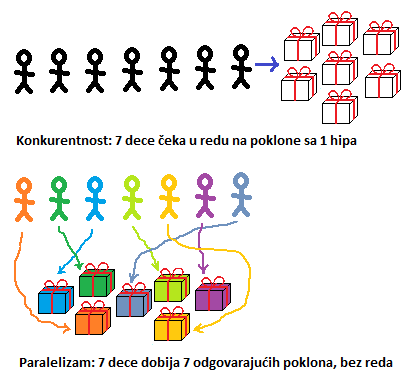
\includegraphics[width=0.6\textwidth]{parallelism-centric.png}
  \caption{Разлика између конкурентног и паралелног израчунавања}
  \label{fig:ParVSCon2}
\end{figure}
% Dve slike jedna pored druge
%\begin{figure}[!tbp]
%  \centering
%  \subfloat[Flower one.]{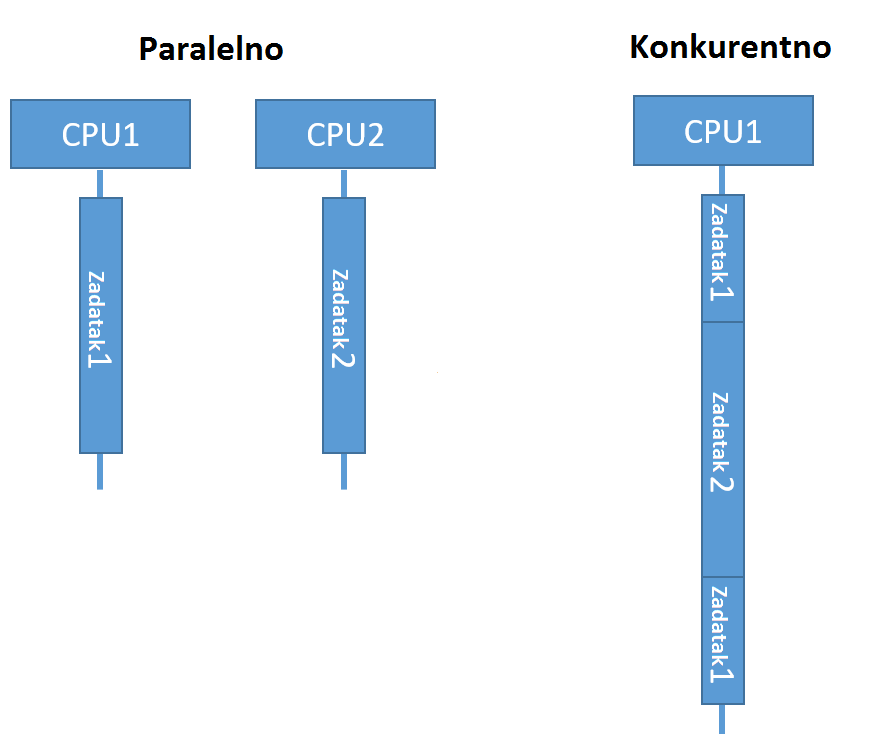
\includegraphics[width=0.5\textwidth]{parallel-vs-concurrent-dotnet-core.png}\label{fig:f1}}
%  \hfill
%  \subfloat[Flower two.]{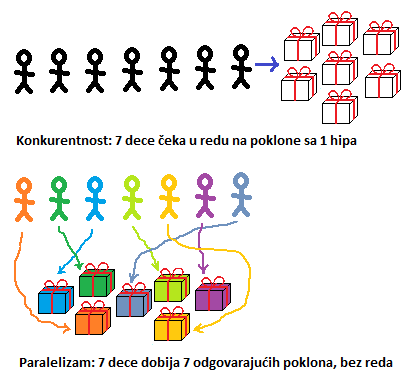
\includegraphics[width=0.5\textwidth]{parallelism-centric.png}\label{fig:f2}}
%  \caption{My flowers.}
%\end{figure}
%
 
Оно што је скупо код конкурентног извршавања је промена контекста (енг. \textit{context switch}) а то је промена стања процесора која је неопходна у случају када процесор са извршавања кода једног процеса прелази на извршавање кода другог процеса. Оваква промена се дешава јако често, до неколико стотина хиљада пута у секунди по процесорском језгру,  што је незгодно јер узима доста процесорског времена. Такође, подаци о стању процеса заузимају много меморије.

То је довело до појаве \textbf{нити} (енг. \textit{thread}). Нит је компонента процеса која се извршава секвенцијално, тако да један процес може имати више нити. Нити омогућавају штедњу што се тиче ресурса ако постоје подаци које те нити деле. Самим тим, добија се и на времену. Нити се, као и процеси, могу извршавати конкурентно и паралелно.

Постоје различити модели тј. стилови паралелног програмирања. Ови стилови говоре о начинима комуникације процесорских језгара, нити, и начинима на који је то остварено. У наставку су објашњена два модела, модел дељења меморије и модел размене порука \cite{survey}.

%---------------
\subsection{Модел дељења меморије}
Рад са нитима подржава модел дељења меморије (енг. \textit{shared memory model}). То значи да нити имају део меморије који им је заједнички, тако да могу асинхроно да читају и пишу на те меморијске локације. Ту се јављају разни проблеми. Треба омогућити безбедно дељење ресурса, комуникацију и синхронизацију нити.  Случајеви када две или више нити не смеју истовремено имати приступ истим подацима су веома чести и зато се прибегава решењима закључавања као што су мутекси, катанци, монитори, семафори. Сврха ових решења је спречити недозвољене приступе подацима који се деле. Некада је дозвољено истовремено читање података, а некада је строго забрањен приступ свим нитима осим оне која тренутно чита и/или мења податке. Такве одлуке се доносе у зависности од конкретног случаја и потреба \cite{progInScala3, survey}.

Механизми закључавања решавају проблеме који се тичу приступа подацима, али уводе нове проблеме \cite{progInScala3}:
\begin{itemize}
\item \textbf{Катанци спречавају састављање} Као што је поменуто, функционални језици охрабрују писање мањих целина од којих свака има јасно дефинисан задатак. Ове мање целине на крају "саставе" цео програм. Ово није могуће ако користимо катанце.
\item \textbf{Превише или премало катанаца} Закључавање и откључавање катанаца представљају скупе операције. Често није јасно колико је катанаца потребно да програм ради како треба а да не утиче на перформансе. Премало катанаца повећава шансу за недозвољеним приступом а са превише њих долази до пада перформанси и мртвих петљи.
\item \textbf{Мртва петља и надметање за ресурсима} Ово су неки од проблема карактеристичних за конкурентно програмирање.

Мртва петља (енг. \textit{deadlock}) или \textit{узајамно закључавање} је ситуација када више процеса или нити уђе у стање чекања због тражења ресурса који није доступан. Све ове нити чекају да им нека друга ослободи ресурс, али је то немогуће јер нит коју чекају такође чека неки ресурс. Пример је дат на слици \ref{fig:deadlock}:
\begin{figure}[!ht]
  \centering
  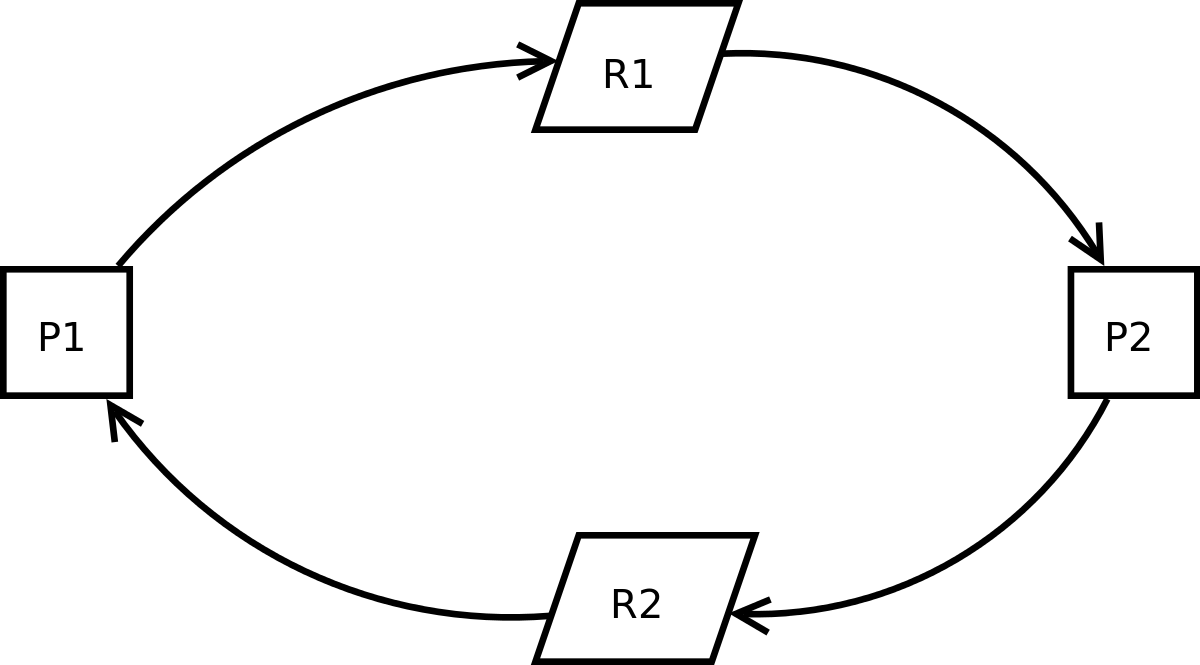
\includegraphics[width=0.5\textwidth]{deadlock.png}
  \caption{Мртва петља}
  \label{fig:deadlock}
\end{figure}
Процес P1 тражи ресурс R1 али не успева да му приступи јер процес P2 држи ресурс R1. Слично, процес P2 тражи ресурс R2 али њега држи процес P1. Два процеса су у застоју јер се међусобно чекају. Проблем мртве петље се може решити тражењем катанаца у унапред дефинисаном редоследу, али и даље представља оптерећење за програмере \cite{microsoftRaceC}.

\label{raceCon}
Надметање за ресурсима (енг. \textit{race conditions}) представља ситуацију када два или више процеса или нити истовремено читају и мењају исти податак. Један од тих процеса поништи измене другог процеса, па резултат који се добије на крају зависи од редоследа којим процеси мењају дати податак. Редослед је немогуће предвидети тако да се приликом покретања оваквог програма углавном сваки пут добије другачији резултат \cite{microsoftRaceC}.

\item \textbf{Тежак опоравак од грешака} Не постоји одређени механизам за опоравак програма са више нити од грешака. Углавном је корисно проћи кроз \textit{.log} датотеку у којој je у различитим тренуцима записанo стање стека са циљем праћења позивања функција и промена вредности променљивих.
\end{itemize}

Писање конкурентних програма је јако тешко. Нити су ниског нивоа, веома блиске хардверу и представљају начин на који сам процесор обавља послове. Постоји мало програмера који су у стању да напишу конкурентан програм без грешака тако да тај посао треба препустити стручњацима у тој области. Један од главних разлога што је ово тежак посао је непредвидивост конкурентних и паралелних програма. Немогуће је утврдити којим редоследом ће се послови обављати, а веома је компликовано доказати да је програм \textit{коректан} тј. да ради управо оно што се од њега очекује. Програмери се ослањају на своје логичко размишљање и надају се најбољим исходима. Друга ствар која је кључни разлог тежине конкурентног програмирања је коришћење променљивих података. Дељени подаци који се временом мењају захтевају синхронизацију и механизме закључавања, отежавајући паралелизацију конкурентног програма. То су разлози због којих је функционална парадигма погоднија од других за паралелизацију. Чим нема мутабилних тј. променљивих структура нема ни проблема које оне носе са собом \cite{progInScala3}.

%---------------
\subsection{Модел размене порука}

Модел размене порука (енг. \textit{message passing model}) је један од нових "трендова" који се тичу конкурентности. Овај модел подржава \textbf{SN} тј. \textit{Shared Nothing} архитектуру. SN архитектура се односи на дистрибуиране системе и подразумева да се систем састоји из неколико независних чворова. Сваки чвор (тј. независна машина) има своју меморију, дискове и интерфејсе за улаз и излаз. Расположиви подаци се поделе овим чворовима тако да сваки од њих има одговорност искључиво за своје податке. Подаци се међу чворовима никада не деле што значи да сваки чвор има потпуну слободу над својим делом па нема потребе за механизмима закључавања. Како се међу чворовима ништа не дели, отуда назив ове архитектуре \cite{SNvsSD, warehouse}.

Оваква логика недељивости стоји и иза модела размене порука. Компоненте овог модела међусобно комуницирају искључиво размењујући поруке. Свака компонента овог модела има своје стање (које јесте променљиво) али га никада не дели са другима, а поруке које шаље су \underline{непроменљиве}. Поруке се могу слати синхроно и асинхроно \cite{progInScala}.

Модел размене порука се може имплементирати на више начина, а најуспешнији начин је помоћу такозваног модела \textbf{Actors}. Њега је осмислио амерички научник Карл Еди Хјуит (енг. \textit{Carl Eddie Hewitt}) који је 1973. године заједно са другим ауторима објавио рад који представља увод у модел Actors. Иако се развија годинама, тек је од скоро доказано да је овај модел ефикасан у решавању проблема савремених рачунарских система. Он енкапсулира тежак рад са нитима и олакшава програмирање конкурентности. 

Компоненте Actor модела представљају објекти које зовемо \textit{Actors}. Они формирају хијерархијску структуру у којој сваки објекат има свог родитеља који сноси одговорност за њега. Сваки Actor има своје "поштанско сандуче" и његов задатак је да обради сваку поруку коју добије. Поруке се чувају у FIFO (енг. \textit{first-in first-out}) структури тј. \textit{реду} (енг. \textit{queue}) па се поруке обрађују редом којим су стигле. Оно што разликује објекте Actor од других објеката је способност реаговања на поруке одређеном акцијом. Као одговор на поруку Actor може направити још Actor компоненти (своју децу), слати поруке другим компонентама или зауставити рад своје деце или себе. Actor има своје локално стање које је променљиво, али са другима не дели ништа осим порука. Важна особина Actor објеката је да се не блокирају када пошаљу поруку већ настављају са радом, односно слање порука је увек асинхроно. 

Предности Actor модела и уопште SN архитектуре се огледају у избегавању свих поменутих проблема конкурентног програмирања чији највећи узрок представљају дељени променљиви подаци. Actor модел је погодан у апликацијама у којима је могуће посао поделити на што више мањих, независних послова. Тада сваки мањи посао представља задатак једне Actor компоненте. Родитељ решава проблеме своје деце и прикупља резултате њихових послова. Дизајн такве апликације личи на организацију послова у компанијама где се послови деле по одељењима, све док ти послови не постану довољно једноставни да их може обавити један радник. 

Иако Actor модел у многим случајевима олакшава посао, постоје ситуације када је неопходно да компоненте деле податке између себе. Не треба на силу користити један модел ако природа проблема намеће неки други. Actor модел није универзално решење за све проблеме већ треба препознати случајеве када га није погодно користити. Неке од ситуација када треба прибећи другачијем решењу су следеће \cite{progInScala3}:

\begin{description}
\item \textbf{Дељени променљиви подаци} Неки проблеми природно захтевају дељење података. Тада је погодније изабрати рад са нитима, поготово ако се подаци деле само за читање. Рад са базама података и трансакцијама је пример када се програмери обично одлучују за неко друго решење.
\item \textbf{Цена асинхроног програмирања} Модел дељења порука са собом носи одређену сложеност. Дебаговање и тестирање великих апликација које имплементирају модел дељења порука може бити веома тешко. Наиме, компликовано је праћење асинхроно послатих порука што доводи до тешког проналаска извора проблема. У овом случају је корисна информација о првој послатој поруци. Такође, многим програмерима је тешко да се навикну на нову парадигму што изискује труд и време.
\item \textbf{Перформансе} Неке апликације захтевају највећу могућу брзину и ефикасност. Иако је Actor модел у већини случајева примењив, нити се налазе на нижем нивоу и самим тим омогућавају боље перформансе. 
\end{description}

Разни језици имају библиотеке које имплементирају Actor модел. У следећем поглављу је обрађена одговарајућа библиотека у Скали \cite{progInScala3, carlHewittActor, seven}.

% ------------------------------------------------------------------------------
\section{Библиотека Akka}
\label{sec:akka}

\textbf{Akka} представља имплементацију Actor модела на Јава виртуелној машини. Од верзије 2.10 језика Скала ова библиотека је подразумевана библиотека за коришћење Actor модела. Постојала је и библиотека \textit{Actor}, али је она застарела и од верзије 2.11 се више не користи \cite{akkaMarius}.

Све што се тиче Actor објеката је смештено у својству \textit{Actor} које се уводи \textit{import} наредбом:
\begin{lstlisting}[language=Scala]
import akka.actor.Actor
\end{lstlisting}

Кључне особине које одликују Actor компоненте су слање и примање порука. То се ради на следећи начин \cite{progInScala3}: 
\begin{itemize}
\item Слање порука се врши позивом метода \textbf{!}:
\begin{lstlisting}[language=Scala]
a ! msg
\end{lstlisting}
Објекту \textbf{a} се шаље порука \textbf{msg}.
\item Примање порука се остварује помоћу \textbf{receive} блока и упаривања образаца које је објашњено у поглављу \ref{uparObr}:
\begin{lstlisting}[language=Scala]
receive {
	case pattern1 => 
		...
	case patternN => 
}
\end{lstlisting}
\end{itemize}

Све компоненте Actor система су хијерархијски распоређене и организоване тако да се свакој приступа на јасно дефинисан начин. Ово је тема следећег поглавља.

\subsection{Структура}
\label{subsec:struktura}

Све Actor компоненте које припадају једној логичкој компоненти апликације (нпр. једна за управљање базом података а друга за реаговање на захтеве корисника) припадају заједничком систему који се назива \textbf{ActorSystem}. То је хијерархијски уређена група компонената које деле исту конфигурацију. На ActorSystem можемо гледати као на менаџера својих компоненти који прави нове и претражује постојеће компоненте. Такође, ActorSystem је задужен за алоцирање $1...N$ нити које ће бити коришћене у апликацији \cite{progInScala3, akkaDoc}.

Све Actor компоненте једног система ActorSystem су смештене у \textbf{стабло} које је приказано на слици \ref{fig:stablo}. Свака компонента има родитеља коме припада. На самом врху хијерархије налазе се три предефинисане компоненте \cite{akkaDoc}:
\begin{itemize}
\item \textit{root guardian} је родитељ свих других компонената. Чак и он интерно има свог родитеља који се назива \textit{"Bubble-Walker"}, али је он невидљив корисницима.
\item \textit{user guardian} је родитељ свих корисничких компоненти (компоненти које су направили сами корисници) и сва његова деца испред свог назива имају префикс "\textit{/user/}".
\item \textit{system guardian} је родитељ свих интерних компоненти. Интерна компонента, на пример, може бити компонента коју направи сама конфигурација оног тренутка када се креира систем ActorSystem. 
\end{itemize}

\begin{figure}[!ht]
  \centering
  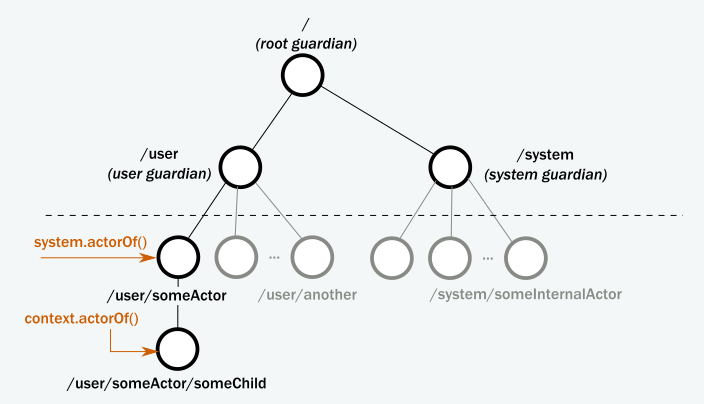
\includegraphics[width=1\textwidth]{akkaTree.png}
  \caption{Стабло Actor компонената}
  \label{fig:stablo}
\end{figure}

Прву компоненту правимо помоћу метода \textit{actorOf} самог система ActorSystem. Све компоненте направљене на овај начин ће постати деца предефинисане компоненте \textit{user guardian}. Овакве компоненте су на врху хијерархије корисничких компоненти, па за њих кажемо да су на највишем нивоу иако постоје предефинисане компоненте изнад њих. Actor компонента која произведе нову компоненту представља њеног родитеља (енг. \textit{parent actor}), а нова компонента је њено дете (енг. \textit{child actor}). Ова радња се постиже методом \textit{actorOf} поља \textit{context} Actor компоненте. Ово поље је типа \textbf{ActorContext} који омогућава једној компоненти да има приступ самој себи, свом родитељу и својој деци. Свако дете добија име свог родитеља као префикс свог имена.

Прављењем Actor компоненте или добијањем постојеће претрагом система не добијамо директну референцу на компоненту, већ добијамо показивач на референцу \textbf{ActorRef}. Ова референца је задужена за слање порука својој компоненти и штити је од директног приступа корисника. Свака компонента има приступ својој референци преко поља \textit{self}, а током обраде примљене поруке преко поља \textit{sender} има приступ референци компоненте која јој је поруку послала.

Оваква хијерархијска структура је слична структури датотека у систему. У систему ActorSystem свака Actor компонента има путању \textbf{ActorPath} која је јединствено идентификује. Пошто се компоненте могу налазити и на више чворова на мрежи тј. извршавати се на различитим Јава виртуелним машинама, први део путање садржи протокол и локацију на којој се налази компонента (идентификацију ActorSystem система у коме се налази). Надаље путању чине надовезани елементи у стаблу раздвојени са "/", почевши од корена. На пример \cite{akkaDoc}:
\begin{lstlisting}[language=Scala]
"akka://my-sys/user/service-a/worker1"                  		   	 // lokalna komponenta
"akka.tcp://my-sys@host.example.com:5678/user/service-b" 	// udaljena komponenta
\end{lstlisting}
Код примера локалне путање протокол је "akka" a ActorSystem je "my-sys". Међутим, нелокална путања дефинише другачији протокол и уз то име домаћина (енг. \textit{host}) и број порта. У обе путање присутне су поменуте компоненте "root guardian" и "user guardian" што чини део путање "/user". Након тога следе корисничке компоненте које добијамо проласком кроз стабло све до жељене компоненте.

Још једна сличност ове хијерархије са хијерархијом система датотека је начин на који претражујемо њене елементе. На пример \cite{akkaDoc}:
\begin{lstlisting}[language=Scala]
context.actorSelection("../*") ! msg
\end{lstlisting}
Метод \textbf{actorSelection} враћа референце компоненти које тражимо путем аргумента. Користећи "\textbf{..}" пењемо се један ниво изнад у стаблу тј. добијамо свог родитеља, а како "\textbf{*}" представља знак за било шта (\textit{wildcard}), добијамо сву децу свог родитеља, укључујући и себе. На овај начин лако шаљемо поруку различитим компонентама истовремено.
%компоненту\footnote{Овде се не мисли на Actor компоненту као у остатку текста, већ на обичан елемент система ActorSystem.}
\\
\par Сваки ActorSystem има "диспечера" тј. елемент који се назива \textbf{MessageDispatcher}. Овај диспечер је задужен за слање порука у одговарајуће поштанско сандуче као и за позивање одговарајућег receive блока Actor компоненте. У позадини диспечера налази се складиште нити која се назива \textit{thread pool}. Складиште садржи одређени број покренутих али неактивних нити које чекају да им се додели задатак. Сваки пут када је потребно извршити нови задатак, проверава се постојање слободне нити у групи. Ако постоји, бира се прва слободна нит. У случају да су све нити тренутно заузете, прва нит која се ослободи ће преузети нови задатак. Оваква идеја се примењује уколико знамо да ће бити пуно нити које ће извршавати кратке задатке, па је ефикасније имати унапред спремне нити него их изнова и изнова правити. На овај начин се такође смањује број нити које се креирају током рада апликације.

\textit{Thread pool} даје важну гаранцију у конкурентној апликацији, а то је да у сваком тренутку само једна нит може извршавати одређену Actor компоненту. То значи да никада две или више нити не могу истовремено извршавати исту компоненту. Једну компоненту могу извршавати различите нити али само у различитим временским интервалима. То нам омогућава да безбедно мењамо податке унутар Actor компоненте докле год те податке не делимо \cite{progInScala3, akkaDoc}. 
\\
\par Компонента која је задужена за примање порука које су послате обустављеној или непостојећој компоненти назива се \textit{dead letter actor}, а њено сандуче \textit{dead letter mailbox}. Након што се одређена компонента угаси, није добра пракса направити нову са истом путањом. Разлог томе је то што не можемо претпоставити редослед догађаја и може се десити да нова компонента прими поруку која је била намењена старој \cite{akkaDoc}.
\\
\par Један од разлога због којих су компоненте смештене у хијерархијску структуру је управљање њиховим животним циклусима. Компоненте живе до момента када их корисник заустави и тада се прво рекурзивно заустављају сва њена деца. Ниједно дете не може надживети свог родитеља. То је корисно јер се на тај начин спречава цурење ресурса. Такође, препоручује се заустављање компоненте једино из ње саме. Добра је пракса да компонента као одговор на одређену поруку заустави саму себе док се заустављање произвољне компоненте из неке друге избегава.

Други разлог постојања хијерархије је управљање грешкама и изузецима. Akka подржава програмирање у коме се стање грешке посматра као било које друго валидно стање. Немогуће је спречити све грешке, тако да је циљ припремити начине на које ћемо се изборити са њима. У томе помаже структура компонената. Када компонента наиђе на проблем она привремено суспендује сву своју децу и саму себе, и обавештава родитеља о проблему. Њен родитељ одлучује како даље наставити са радом. Другим речима, сваки родитељ је задужен за решавање грешака и изузетака своје деце и тиме представља њиховог \textit{супервизора}. Акција коју родитељ одлучи да предузме назива се \textit{стратегија супервизора} (енг. \textit{supervisor strategy}). Подразумевана стратегија је заустављање и поново покретање (рестартовање) детета и оно подразумева брисање акумулираног стања и враћање на почетак. Ову акцију је могуће предефинисати, тако да поред рестартовања постоје још три опције које родитељ може предузети \cite{progInScala3, akkaDoc}:
\begin{enumerate}[1)]
\item Настављање са радом са акумулираним стањем
\item Трајно заустављање детета
\item Пропагирање грешке на ниво изнад тј. обавештавање свог родитеља о њој и тиме суспендовање себе
\end{enumerate}

Што се тиче самог рестартовања, разликујемо две стратегије: \textit{One-for-One} и \textit{All-for-one}. Ове стратегије говоре о томе шта се дешава са осталом децом супервизора тј. родитеља компоненте која се рестартује и илустроване су на сликама \ref{fig:oneForOne} и \ref{fig:allForOne} \cite{progInScala3, akkaDoc}:
\begin{itemize}
\item \textbf{One-for-One} је подразумевана стратегија у којој током рестартовања одређене компоненте остале поменуте компоненте живе и настављају са радом независно од ње. Ова стратегија се примењује када компонента врши посао који не утиче на послове других компоненти.
\item \textbf{All-for-One} стратегија се примењује када компоненте заједно учествују у неком послу тако да рестартовање једне повлачи рестартовање и осталих компоненти. У овом случају рестартовање једино компоненте у којој се јавила грешка не би било валидно.
\end{itemize}

\begin{figure}[!tbp]
  \centering
  \subfloat[One-for-One]{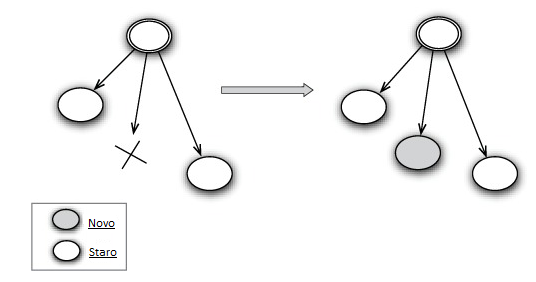
\includegraphics[width=0.5\textwidth]{oneForOne.png}\label{fig:oneForOne}}
  \hfill
  \subfloat[All-for-One]{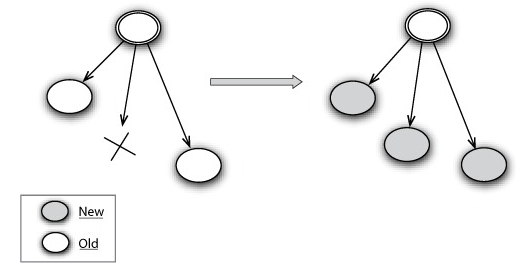
\includegraphics[width=0.5\textwidth]{allForOne.png}\label{fig:allForOne}}
  \caption{Стратегије рестартовања}
\end{figure}

%\subsection{Future и Promise објекти}
%\label{subsec:futPro}

%--------

% ------------------------------------------------------------------------------
\chapter{Расплинуто тестирање}

Грешке у раду било које природе су неминовне, па тако и у програмирању. Развојем софтвера развијају се нове врсте пропуста. "Постоје стотине слабости софтвера које само чекају да буду откривене, и биће откривене када прође довољно времена" \cite{fuzzing}. Неке грешке немају велики значај док друге могу оставити озбиљне последице. Постоје програми који користе грешке других програма уметањем вируса, црва, злонамерних скриптова и слично. Циљ напада на софтвер може бити преузимање или пад система, крађа, злоупотреба и мењање постојећих података, производња нових и лажних података итд.  Зато је јако важно софтвер тестирати са циљем елиминисања што већег броја грешака које могу угрозити квалитет и безбедност система. \cite{fuzzing, bezbMalkov}.

Расплинуто тестирање (енг. \textit{fuzz testing/fuzzing}) је приступ тестирању софтвера који се бави генерисањем великог броја улаза у програм а затим за сваки од улаза посматра његов ток извршавања. Циљ ових улаза је да открију необичне грешке и изузетке у програму. Улази треба да буду неочекивани и генеришу се или потпуно случајно или уз коришћење одређених \textit{хеуристика}. Узимају се у обзир и неисправни улази јер је важно да програм препозна и одбаци овакве улазе без прекида или отежавања даљег рада. %"Расплинуто тестирање на своју мету баца све осим кухињске судопере и посматра резултате" %\cite{fuzzingBrute}. 

\section{Основе тестирања софтвера}

Тестирање софтвера представља најчешћи вид верификације софтвера. \textit{Верификација} софтвера се бави испитивањем исправности програма тј. провером жељеног понашања програма задатог \textit{спецификацијом}. Постоје \textit{статичка} и \textit{динамичка} верификација. Статичка испитује исправност програма без извршавања кода тј. његовом анализом, док динамичка подразумева испитивање у току извршавања кода \cite{milenaDokt}. 

Тестирање се може описати на више начина. Често се описује као процес коме је циљ процена квалитета софтвера. Овакву дефиницију тестирања треба узети са резервом. Тестирање нам свакако даје увид у квалитет софтвера али прилично мали, јер углавном случајеви које тестирамо представљају само кап у океану свих могућих случајева. Мање амбициозна дефиниција представља тестирање као процес који покушава да открије грешке у програму посматрајући његово извршавање у контролисаним условима \cite{testPrinc}.

Технике тестирања софтвера константно напредују, али треба имати у виду њихова ограничења. Холандски информатичар и добитник Тјурингове награде Едсгер Дајкстра (хол. \textit{Edsger Wybe Dijkstra}) је рекао: "Тестирање софтвера може показати присуство грешака, али никада њихово одсуство" \cite{testPrinc}. Тестирање не може доказати исправност софтвера, већ се за то користе друге, математичке технике. Ипак, тестирање има важну улогу у свим фазама развоја софтвера. Помоћу њега смањујемо број промаклих грешака и повећавамо поузданост изграђеног система.

Због ефикасности процеса тестирања, често је пожељна његова аутоматизација. Генерисање тест примера је у већини случајева потребно извршити ручно, мада постоје неке врсте тестирања у којима је могуће аутоматизовати овај процес. Што се тиче извршавања тест примера, аутоматизација је углавном могућа и њу подржавају разни алати за развој софтвера.

Важно је на који начин се приступа тестирању софтвера. Некада је дизајн тестова једнако компликован као дизајн самог програма. Било да се тестирање врши ручно или аутоматизовано, пожељно је имати планове и идеје о тест примерима који су вероватнији да изазову грешку од других. Треба одредити и редослед којим ће се извршавати осмишљени тестови. Редослед је важан јер постоје случајеви када се одређени тест примери не могу извршити пре извршавања неке друге радње. Рецимо, не можемо тестирати брисање податка из базе података ако је она празна тј. ако претходно није успео тест уметања податка у базу. Након извршавања тестова прегледају се добијени резултати и утврђује се спремност тестираног система. Сав посао везан за тестирање може вршити сам програмер који је уједно и тестер. Друга могућност је постојање тестера који поред програмирања разуме технике тестирања, познаје грешке које се често јављају и необичне случајеве који их производе. Он може да ради заједно са програмером а може бити и раздвојен од њега \cite{guideTestDesign, testMilena}.

"Покривеност кода (енг. \textit{code coverage}) је број неких елемената програма испитаних тестовима у односу на укупан број тих елемената" \cite{testMilena}. Уопштено, покривеност представља неку врсту метрике која говори о броју случајева који су испитани тестовима. Када сматрамо да тестови испитују добар део програма, кажемо да тестови "покривају" велики број случајева тј. да имају велики ниво покривености. У зависности од изабраних елемената програма разликујемо покривеност путања, наредби, грана/одлука, услова, вишеструких услова и функција. Постоје различити алати за рачунање нивоа покривености кода \cite{testMilena}.
%-------------
\subsection{Нивои тестирања}
\label{subsec:nivoiTest}

\par Тестирање се врши на више нивоа, у зависности од сложености компонената које се тестирају. Почиње се од \textbf{тестирања јединица кода} (енг. \textit{unit testing}), тј. независних делова система. Јединице представљају најмање независне целине које обављају неку функцију (нпр. класа или функција). Пре спајања више независних јединица, важно је да оне саме раде правилно, изоловане од других јединица. Други ниво, \textbf{компонентно тестирање} (енг. \textit{component testing}), је веома слично првом нивоу. Компоненте су изоловане од других компонената, али су мало веће и јединице које су у њима нису изоловане једне од других. Трећи ниво је \textbf{интеграционо тестирање} (енг. \textit{integration testing}). Оно је задужено за тестирање компоненти које заједно чине целину система. То је важно јер се неретко дешава да компоненте које савршено раде самостално не успевају добро да раде заједно и комуницирају једне са другима. Следећи ниво тестира систем као целину и зато се назива \textbf{системско тестирање} (енг. \textit{system testing}). На овом нивоу се тестира и хардвер, а тестирање не обухвата само функционалност програма већ и безбедност, капацитет, перформансе, преносивост, итд. На овом нивоу се примењује \textbf{истраживачко тестирање} (енг. \textit{exploratory testing}) током кога тестер извршава тест случајеве који нису били у плану, са намером да открије непредвиђене начине коришћења система. Обављају се и \textbf{тестови прихватљивости} (енг. \textit{acceptance testing}) које извршавају корисници, проверавајући да ли софтвер испуњава њихова очекивања и потребе. Након измена система врши се \textbf{регресионо тестирање} (енг. \textit{regression testing}) које треба да покаже правилан рад неизмењених  функција. Такође треба да покаже и да су перформансе новог система макар једнаке перформансама старог система, а пожељно је да су боље. Сви ови нивои се примењују уколико време дозвољава темељно тестирање. У случају мањка времена, тестирање се прилагођава могућностима \cite{guideTestDesign, testMilena}.

%-------------
\subsection{Стратегије тестирања}
\label{subsec:stratTest}

На основу доступних информација о имплементацији софтвера који се тестира разликујемо три основне стратегије тестирања \cite{fuzzingBrute, fuzzing, testMilena}: 

\begin{description}
\item \textbf{Тестирање беле кутије} (енг. \textit{white box testing}) или \textit{структурно} (енг. \textit{structural testing}) тестирање подразумева познавање интерне структуре и имплементације програма. Тестерима је доступан целокупан изворни к\^{о}д, тако да је њихов посао да га детаљно изуче како би нашли делове који су подложни грешкама. То је мукотрпан посао јер подразумева пролажење кроз све линије кода којих често има превише за људску обраду. Због тога се углавном користе алати који скенирају к\^{о}д и региструју потенцијалне слабости програма. Након тога их проверава програмер и одлучује да ли су пронађене слабости заиста претња. Алати много помажу али не могу да замене знање и искуство стручњака. 
\par Добра страна ове стратегије је што доступност изворног кода омогућава високу покривеност кода (можемо проћи кроз велики број путања кроз програм, кроз много грана, итд.). Ипак, велики број линија кода повлачи и велику сложеност његовог анализирања. Алати који анализирају к\^{о}д често окарактеришу пуно делова кода као потенцијалне слабости. Тада програмери морају проћи кроз дугачак извештај о њима, а углавном се испостави да је већина записаних слабости лажна узбуна. Такође, ова стратегија је непримењива уколико изворни к\^{о}д није доступан. Треба имати у виду да је доступност кода уобичајена код програма на Linux оперативним системима, што није случај код програма писаних за Windows оперативне системе. 

\item \textbf{Тестирање црне кутије} (енг. \textit{black box testing}) или \textit{функционално} (енг. \textit{functional testing}) не користи никакве информације о интерној структури и имплементацији програма. Ова стратегија се може применити када информације о унутрашњој структури нису доступне, али је корисна и када јесу доступне, поред тестирања беле кутије. Једине информације које се користе су улаз и излаз из програма. Тестирање се углавном заснива на претпоставкама о тестираном програму, његовим спецификацијама и налажењу прихватљивог броја репрезентативних тест примера.
\par Једна од предности ове стратегије је примењивост. Без обзира на доступне информације, тестирање црне кутије је увек могуће и једноставније од осталих стратегија јер не изучава специфичности одређеног програма. Погодно је јер га могу примењивати и тестери који нису програмери. Такође, због тога што се тестови не ослањају на унутрашњу структуру софтвера, исти тест можемо употребљавати више пута за различите програме сличне намене. Једноставност овог приступа има и своје мане. Пошто се тестирање врши на основу претпоставки, никада не можемо тачно проценити ефикасност тестирања и ниво покривености кода као код тестирања беле кутије. Такође, ова стратегија није погодна за комплексне нападе где је потребно извршавати тестове одређеним редоследом ради изазивања рањивог стања програма.

\item \textbf{Тестирање сиве кутије} (енг. \textit{gray box testing}) представља комбинацију претходне две стратегије. Једна могућност је да се тестови базирају на обема техникама беле и црне кутије. Друга могућност је да у некој мери постоје информације о унутрашњој структури софтвера, али не као код тестирања беле кутије. Изворни к\^{о}д није доступан али се увид у структуру софтвера добија преко датотека компајлираног програма тј. његових бинарних извршних датотека. Како су ове датотеке нечитљиве за људе, на њих се примењује процес обрнутог инжењеринга (енг. \textit{reverse engineering}). Обрнути инжењеринг не може да открије изворни к\^{о}д програма, али препознавањем одређених инструкција може да произведе формат који се налази између изворног кода и машинског кода. За разлику од бинарних датотека, овај формат је читљив за људе и омогућава анализу сличну као код структурног тестирања. 
\par Тестирање сиве кутије је хибридно решење које може искористити предности стратегија црне и беле кутије. Уколико изворни к\^{о}д није доступан, често се користи обрнути инжењеринг као допуна чистом тестирању црне кутије. То је могуће јер су бинарне датотеке софтвера увек доступне (осим Веб сервера и апликација). Мана ове стратегије је велика сложеност обрнутог инжењеринга који захтева постојање богатих ресурса.
\end{description}

Свака од поменутих стратегија има своје предности и мане. Ни за једну се не може рећи да је генерално боља од других, јер је свака од њих погодна за откривање различитих врста слабости. Најбоље решење је применити више стратегија ради откривања што више грешака. Различитост стратегија илустрована је сликом \ref{fig:boxes}.

\begin{figure}[!ht]
\centering
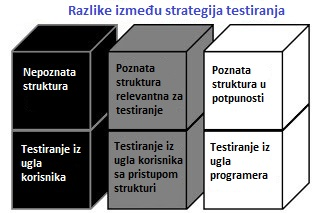
\includegraphics[width=0.5\textwidth]{boxes.jpg}
\caption{Разлике између стратегија тестирања}
\label{fig:boxes}
\end{figure}
% (енг. \textit{})

\section{Основе расплинутог тестирања}

Развојем расплинутог тестирања је откривено доста начина генерисања улаза који у великом броју случајева откривају грешке. Најчешће се улази или делови улаза генеришу случајно, праве се улази који су мањи него што би требало (нпр. датотека са мање података), користе се негативне и граничне вредности нумеричких типова података, предугачке ниске карактера, ниске карактера са специјалним карактерима, замењују се суседни битови, итд. Не постоје правила која дефинишу радње које се примењују на подацима, већ само савети који су експериментално откривани годинама.  

Кључна предност расплинутог тестирања наспрам других техника тестирања је могућност аутоматизације овог процеса. Ручно креирање тест примера и покретање програма је веома напорно, споро, неефикасно и захтева да га обавља стручњак у области тестирања. Зато се прибегава аутоматизацији што је могуће већег дела посла које тестирање захтева. Тестирање може покренути особа без великог знања о томе. Такође, многе апликације за тестирање су примењиве на велики број различитих програма \cite{fuzzingBrute, fuzzing}.

Расплинуто тестирање је један од приступа тестирања црне кутије. Програм за тестирање не зна ништа о структури програма који тестира. Проблем који се јавља оваквим тестирањем је тај што формирани улази често откривају грешке које је лако открити јер се тај део кода често извршава,  док семантичке грешке које се налазе дубоко у програму остају неоткривене. Зато су развијени приступи алтернативног расплинутог тестирања који одговарају тестирању црне, беле и сиве кутије \cite{fuzzing, grayBoxFuzzing, whiteBoxFuzzing}:
\begin{description}
\item\textbf{Расплинуто тестирање црне кутије} (енг. \textit{black box fuzzing}) је стандардни приступ на који се мисли под појмом "расплинуто тестирање". Он је најлакши за имплементацију и омогућава тестирање великог броја тест примера за кратко време. Показује се да је често ефикаснији од других приступа уколико њима треба превише времена за генерисање тест примера.
\item\textbf{Расплинуто тестирање беле кутије} (енг. \textit{white box fuzzing}) пре самог тестирања користи технике које идентификују делове програма који могу да имају грешке. На тај начин ова врста тестирања повећава покривеност кода, открива грешке до којих се теже долази него другим врстама тестирања, али је и компликованија од њих. 
\item\textbf{Расплинуто тестирање сиве кутије} (енг. \textit{gray box fuzzing}) је приступ који има предности претходне две технике а труди се да избегне њихове мане. Тежи се да ефикасност буде што ближа ефикасности приступа црне кутије, али ова техника не генерише улазе "на слепо" већ користи неки паметнији начин, као приступ беле кутије. Уместо анализе кода, користe се технике инструментације да се добије увид у структуру програма.
\end{description}

\subsection{Историја}
\label{subsec:history}

Примена тестирања налик на расплинуто је почело још 1980-их година са алатом званим "мајмун" (енг. \textit{"Тhe monkey"}). Он је развијен за тестирање програма на Macintosh рачунарима, који су имали проблема због мањка меморије. Мајмун је симулирао правог мајмуна који неартикулисано удара у тастатуру и миш рачунара и на тај начин тестира рад покренутог програма. Ипак, до 1990-их су интересовања и потребе за тестирањем биле много мање него данас, највише због недостатка интернета и идеја напада на други софтвер. Истраживање безбедности софтвера је почело крајем 1980-их година, када су почели да се развијају напади који се односе на прекорачење бафера. Један од познатих напада је настао 1988. године и назива се "Morris Internet Worm" \cite{fuzzingBrute, fuzzing}. 

Први пројекат развијен за тестирање је написан 1989. године. Идеју за овај пројекат је добио професор Бартон Милер (енг. \textit{Barton Miller}), за кога неки сматрају да је "отац" расплинутог тестирања. Заједно са својим ученицима са курса о оперативним системима тестирао је квалитет и поузданост UNIX апликација. Програм је случајно генерисао ниске карактера и прослеђивао их апликацијама. Иако је тестирање имало веома једноставну идеју, у то време је то био велики помак јер се о расплинутом тестирању знало јако мало. На Универзитету у Оулу у Финској је 1999. године почело развијање пакета тестова под називом \textbf{PROTOS}. Ови тестови су проверавали безбедност разних протокола. Компанија Microsoft је 2002. године новчано помогла овој иницијативи тако да је тим који је развијао PROTOS 2003. године засновао компанију за производњу пакета тестова, под именом \textbf{Codenomicon}. Након тога, објављен је програм за тестирање отвореног кода имена \textbf{SPIKE}. Он је био напреднији од програма који је развио професор Милер. Брзо је почело и развијање других пројеката попут sharefuzz, mangleme, Hamachi, CSSDIE, FileFuzz, SPIKEfile, notSPIKEfile, итд. Компанија Mu Security je 2005. године почела да развија хардверски уређај коме је циљ мењање података који се шаљу протоколима путем мреже. ActiveX контроле су такође постале мета програма COMRaider и AxMan 2006. године \cite{fuzzingBrute, fuzzing}. Временом је потреба за сигурношћу софтвера постајала све већа, тако да су се развијали алати за најразличитије врсте апликација. Методе тестирања, као и апликације које врше тестирање, се и данас развијају и побољшавају. Доступан је велики број алата који примењују најновије технике тестирања и врше разне оптимизације ради веће ефикасности. Оптимизације омогућавају краће време и цену тестирања, једноставност коришћења, минималну људску интеракцију, итд. Неки од алата имају специфичну примену, док су други употребљиви у свакој врсти софтвера. Неки од познатијих алата су AFL, Project Springfield, OSS-Fuzz, libFuzz, BFuzz, Fuddly, Honggfuzz, Peach, Radamsa, итд \cite{bestFuzzers, fuzzingBrute, fuzzing}. 

\subsection{Ограничења}
\label{subsec:ogranicenja}

Различите врсте тестирања откривају различите врсте слабости. Не постоји универзална техника за откривање свих грешака, већ у зависности од потреба бирамо одређену технику. Неке од врста проблема које расплинуто тестирање обично не открива су \cite{fuzzingBrute}:
\begin{description}
\item \textbf{Права приступа} Неки програми разликују обичне од привилегованих корисника који имају више права од обичних (рецимо поред читања података могу да их бришу или мењају). Програм за расплинуто тестирање не зна ништа о логици програма који тестира, због чега не разликује типове корисника. Извршавање недозвољених функција од стране обичног корисника ће проћи неопажено код програма за расплинуто тестирање. Могуће је уметнути логику програма у програм за тестирање, али је то веома сложен процес.  
\item \textbf{Дизајн програма} Неки програми имају мане које се односе само на јако лоше осмишљен дизајн. Пример је апликација која дозвољава свим корисницима приступ одређеним подацима. Велика је грешка не узимање у обзир злонамерне кориснике и претпостављање да ће једино корисници који имају дозволу да приступе подацима то и учинити. Проблем је непостојање аутентикације и ауторизације. Програм за расплинуто тестирање не може да препозна овакав безбедносни проблем.
%\item \textbf{Задња врата} ????????
\item \textbf{Корупција меморије} Једна од врста напада на софтвер може бити приступање недозвољеној меморији. Читањем и писањем на разне меморијске локације нападач може имати одређену контролу над програмом. Недозвољен приступ меморији се препозна на нивоу инструкције машинског кода, након чега се програму пошаље сигнал \textit{SIGSEGV}. Проблем је у томе што неретко програми сами решавају овај проблем тако што "ухвате" сигнал и реше да ли да процес покрену поново или само наставе са радом, што може бити опасно. Програм за расплинуто тестирање често не примети овакву врсту слабости јер је она решена (правилно или неправилно) од стране самог програма.
\item \textbf{Сложени напади} Расплинуто тестирање је корисно за детекцију индивидуалних слабости. Међутим, није се добро показало у случају сложених напада који искоришћавају више слабости истовремено.
\end{description}

\section{Врсте програма расплинутог тестирања}
\label{subsec:metode}

Програми расплинутог тестирања се могу међусобно разликовати у доста ствари. Две основне поделе ових програма се односе на начин на који генеришу тест примере и на тип самог програма који тестирају.
Постоје два основна критеријума која говоре о начину на који програм за тестирање генерише улазе у програм.
Први критеријум представља постојање почетних тест примера од којих се генеришу нови тест примери \cite{fuzzingBrute, fuzzing}:
\begin{itemize}
\item \textbf{Тестери засновани на мутацијама} (енг. \textit{mutation-based fuzzers}) користе постојеће тест примере за генерисање нових, примењујући измене тј. мутације на подацима. Квалитет тестирања зависи од квалитета постојећих тест примера. Ови тестери су обично тестери опште намене. 
\item \textbf{Тестери засновани на генерацијама} (енг. \textit{generation-based fuzzers}) генеришу тест примере "од нуле" тј. независно од постојећих. Једине информације које користе су информације о формату који тест примери треба да испоштују (нпр. формат датотека или одређени протокол). Обично су овакви тестери специфични за одређени проблем.
\end{itemize}

Програми расплинутог тестирања, независно од тога да ли су засновани на мутацијама или генерацијама, у некој мери користе случајне податке за генерисање тест примера. Могуће је све податке генерисати случајно, што доводи до тежег увиђања тачног низа догађаја који је довео до грешке. Друга могућност је да се на основу спецификације програма креирају тест примери који ће тестирати граничне вредности података, које су често критичне. Најбоље резултате даје генерисање тест примера комбинацијом ове две могућности.

Мутацијски и генерацијски тестери су основни типови тестера. Поред њих постоји још један тип тестера који се заснива на напредној техници која се назива \textbf{еволуционо расплинуто тестирање} (енг. \textit{evolutionary fuzzing}). Ова техника се заснива на "учењу". На основу претходних корака, тестер закључује које тест примере би требало даље да конструише. Рецимо, за сваки тест пример тестер може да измери покривеност кода, и закључи на који начин да измени тест пример тако да покривеност буде већа. Еволуционо тестирање се ослања на друге технике, попут техника генетских алгоритама \cite{fuzzing, 15minuteGuide}.

Други критеријум који дели програме за тестирање на основу генерисања тест примера је присуство или одсуство знања о томе како треба да изгледају улази у програм који се тестира \cite{fuzzingBrute, fuzzing}:
\begin{itemize}
\item \textbf{Интелигентни тестери} (енг. \textit{intelligent fuzzers}) познају структуру улазних података програма који се тестира. На тај начин се избегне генерисање података које би програм одбацио пре било каквог рада над њима. Имплементација интелигентног тестера је компликована јер захтева проучавање структуре података који представљају улазе у програм.
\item \textbf{Неинтелигентни тестери} (енг. \textit{non-intelligent}/\textit{dumb fuzzers}) конструишу улазне податке у програм "на слепо" тј. не знајући ништа о структури тих података. На тај начин тестер може генерисати велики број улаза који ће брзо бити одбачени од стране програма.
Њихова имплементација је једноставнија од имплементације интелигентних тестера.
\end{itemize}

Ако улаз у програм представља датотека одређеног формата, неинтелигентни тестер генерише тест примере тако што инвертује произвољне битове те датотеке. Са друге стране, интелигентни тестер намерно оставља неке делове датотеке неизмењеним а друге делове мења. Рецимо, ако структуру чине називи поља и њихове вредности, називи ће остати исти док ће се вредности мењати.

Интелигентни тестери углавном имају већу покривеност кода и укажу на већи број грешака од неинтелигентних, али то није правило. Најбоље је креирати тестер који не иде ни у једну крајност, јер то води до лоших резултата. Тестер који не зна ништа о формату улаза уме да креира бескорисне тест примере, али уме и да пронађе неочекивану слабост система да се носи са неисправним улазима. Са друге стране, интелигентни тестер избегава губљење времена непотребним тест примерима, али води до претпостављања правилног рада неких функција система. Неретко се деси да овакав тестер не ради добро јер прави исте претпоставке које је правио и програмер који је писао програм, због којих и долази до одређених грешака. Такође, интелигентни тестер може бити превише скуп због своје сложености. Балансиран приступ је најбоље решење: направити тестер који је довољно интелигентан да смањи време извршавања програма, али да не буде превише сложен и скуп, као и да не ослаби способност тестирања.
%%%%%%%

Неки аутори поистовећују тестере засноване на мутацијама са неинтелигентним тестерима, а тестере засноване на генерацијама са интелигентним тестерима. Такво поистовећивање није исправно. Тестери засновани на мутацијама најчешће заиста јесу неинтелигентни јер обично не узимају структуру улаза у обзир 
већ мењају битове постојећих улаза. Ипак, то није правило. Постоје и интелигентни тестери засновани на мутацијама који парсирају постојеће улазе да не би креирали оне које би програм одмах одбацио.
Слично, тестери засновани на генерацијама могу бити неинтелигентни, иако је то веома редак случај. Рецимо, тестер који генерише улазе случајним подацима, без постојећих улаза, технички спада у тестере засноване на генерацијама. 

% ******************************

У односу на програм који тестирамо, програм за расплинуто тестирање спада у неку од следећих категорија \cite{fuzzingBrute, fuzzing}:
\begin{description}
\item \textbf{Локални тестери} (енг. \textit{local fuzzers}) Ово је веома широка категорија која обухвата тестирање разних локалних програма. Класичан пример програма који су погодни за расплинуто тестирање су програми који омогућавају обичном кориснику да привремено (за време његовог извршавања) добије одређене привилегије. На Unix системима има неколико таквих подразумеваних апликација (енг. \textit{setuid applications}) а то се може подесити и за друге. Слабости у оваквим програмима представљају велику опасност јер би грешкe моглe да омогућe кориснику да трајно добије привилегије и извршава произвољан к\^{о}д. Расплинуто тестирање проналази слабости ових апликација тако што их покреће са трансформисаним аргументима. Аргументи се могу слати програму у виду аргумената командне линије (енг. \textit{command-line fuzzers}), у виду променљивих окружења (енг. \textit{environment variable fuzzers}), или у виду датотека одређеног формата (енг. \textit{file format fuzzers}).
\item \textbf{Тестери удаљених програма} (енг. \textit{remote fuzzers}) Ови тестери се баве програмима који су доступни путем мреже, што је посебно значајно због широке употребе интернета. Међу њима постоје три врсте тестера. 

Прву врсту чине тестери мрежних протокола (енг. \textit{network protocol fuzzers}). Тестирају се једноставни и сложени протоколи. Једноставни су они који имају слабу аутентикацију или је уопште немају, користе ASCII карактере уместо бинарних података, итд. Сложени протоколи се састоје углавном из бинарних података међу којима се налази понекa ASCII ниска карактера. Аутентикација је сложенија и користи шифровање. Такође, често се врше провере помоћу дужине или збира послатих података.  

Другу врсту чине тестери Веб апликација (енг. \textit{Web application fuzzers}). Они комуницирају помоћу HTTP протокола. Веома су важни јер данас имамо јако много апликација на Вебу с којима су се развиле и слабости јединствене за њих попут уметања SQL упита (енг. \textit{SQL injection}), уметање скриптова (енг. \textit{cross site scripting}), онемогућавања услуге (енг. \textit{denial of service}) и многих других.

Последњу врсту чине тестери Веб прегледача (енг. \textit{Web browser fuzzers}). Они спадају у тестере формата датотека али се због важности издвајају као посебна врста. Поред парсирања \textit{html} датотека, могу радити и са \textit{css} датотекама, а и са различитим објектима (рецимо \textit{Component Object Model} објекти који се могу отворити у прегледачу \textit{Microsoft Internet Explorer}). Важна особина им је могућност потпуне аутоматизације.
\item \textbf{Меморијски тестери} (енг. \textit{in-memory fuzzers}) Ови тестери су корисни када су неке друге врсте неефикасне. Њихове идеје су једноставне и заснивају се на измени аргумената функција програма директно у меморији, при чему се мењају и аргументи који иначе нису доступни кориснику. Имплементације оваквих тестера су веома компликоване. Постоји више приступа оваквом тестирању. Један приступ подразумева замрзавање процеса и чувања његовог тренутног стања које се касније поново користи тј. изазове се без поновног покретања процеса. Након тога, у свакој итерацији се у процес у таквом стању уметну неисправни улазни подаци, посматра се резултат и враћа се на сачувано стање. На овај начин се добија на брзини и ефикасности јер се делови програма који су неважни за тестирање прескачу (замрзавањем стања нас не занима шта се и како се извршило пре тога), и одмах се долази до критичног дела. Ипак, ово је веома сложен процес. Могуће је у програм уметнути улазне податке који не би били могући при нормалном покретању програма. Такође, ако се дошло до грешке оваквим тестирањем, потребно је ту грешку изазвати и нормалним покретањем програма, што може одузети доста времена.
\end{description}

\section{Расплинуто тестирање формата датотека}
\label{sec:rasTestFormFajl}

Расплинуто тестирање формата датотека  је метода тестирања апликација које прихватају специфичне улазе. Улази су одређеног формата, тако да је циљ тестирања откривање грешака при парсирању улазних датотека. Примери су програми за манипулацију сликама, документима, музиком, итд. Програми су углавном на клијентској страни, али могу бити и на страни сервера (нпр. сервери електронске поште).

Особина овакве врсте тестирања која је чини једноставнијом од тестирања неких других типова апликација је та што се углавном извршава целокупно на једном систему. Рецимо, у случају  тестирања мрежних протокола или Веб апликација постоје барем два система: један на ком се налази програм који се тестира, и други на ком се покреће тестирање. Са друге стране, тестер формата датотека теже препознаје да је циљана апликација изазвала грешку или изузетак. При тестирању програма на серверу је најчешће очигледно када је дошло до грешке јер сервер постане недоступан. То није случај код клијентских апликација јер програм за тестирање изнова поново покреће апликацију са новим тест примерима. Без адекватног решења може да се деси да тестеру промакне важна слабост програма. Због тога је важно да тестер формата датотека надгледа програм који тестира помоћу постојећег дебагера или дебагера који је уметнут у сам програм за тестирање. То повећава сложеност тестирања формата датотека \cite{fuzzingBrute, fuzzing}.

Тестирање се може описати помоћу следећих пет корака \cite{fuzzingBrute}:
\begin{enumerate}
\item Припремити тест пример методом заснованом на мутацијама или методом заснованом на генерацијама
\item Покренути циљну апликацију и учитати припремљен тест пример
\item Надгледати циљну апликацију (најчешће коришћењем дебагера)
\item У случају откривања грешке, забележити све потребне информације о њој. Ако након одређеног времена ниједна грешка није пронађена, ручно угасити циљну апликацију. 
\item Поновити дате кораке.
\end{enumerate}

Расплинуто тестирање формата датотека може бити интелигентно и неинтелигентно, као што може користити и обе методе засноване на мутацијама и генерацијама. У наставку су описане најчешће коришћене две технике и њихове добре и лоше стране \cite{fuzzingBrute}: 
\begin{description}
\item \textbf{Неинтелигентно расплинуто тестирање засновано на мутацијама} представља веома једноставан приступ чији квалитет зависи од квалитета почетних улаза. Наредни улази се добијају мењањем постојећих, па је важно имати међусобно различите почетне улазе да би што више случајева било покривено. Мењање улаза може бити у виду мењања појединачних бајтова, скупа бајтова, додавањем нових података, итд. Проблем код овог приступа је то што програми пре рада са улазним подацима често проверавају њихову исправност методама као што је провера контролне суме (енг. \textit{checksum}). Улазни податак који је промењен не пролази проверу и бива брзо одбачен од стране програма. Због оваквих провера, тестер успева да испита јако мали део кода. Ово се може решити искључивањем провера што је тежак посао. Такође, овај приступ није ефикасан јер је број свих могућих начина на које можемо променити улазни податак превелик. Могуће је тестирати мали број могућности. Добра страна овог приступа је веома мала количина труда потребна пре покретања тестера, а она се односи на избор почетних тест примера. 
\item \textbf{Интелигетно расплинуто тестирање засновано на генерацијама} је приступ који генерише тест примере на основу шаблона формата датотеке који се користи у тестирању. Шаблон многих формата датотека је познат и може се лако наћи, док у случају непостојања шаблона програмер мора сам проучити дати формат датотека. Квалитет тестирања зависи од тога колико добро програмер познаје дати формат датотека, због чега се много времена улаже у његово проучавање. Проучавање одузима доста времена, али је овај приступ ефикаснији јер тежи покривању већег дела кода.
\end{description}

При парсирању неисправних датотека се може наићи на разне врсте грешака. Неке од најчешћих врста грешака које покушавамо да откријемо расплинутим тестирањем су \cite{fuzzingBrute, fuzzing}:
\begin{description}
\item \textbf{Онемогућавање услуге} (енг. \textit{denial of service}) Ово је напад на систем у коме се онемогућава његов рад. Нападач преоптерећује систем тако што му шаље јако велики број захтева. Системи подложни овом нападу су апликације на серверу.   
\item \textbf{Проблеми у раду са целим бројевима} Цели бројеви су подложни грешкама које се односе на прекорачење меморије. Разлог за то неретко буде знак целих бројева. Јављају се грешке при алокацији меморије, радом са индексима низова, поређењем означених и неозначених целих бројева, итд.
\item \textbf{Прекорачење стека и хипа} До прекорачења меморије било на стеку или на хипу долази из много разлога. Типичан пример подразумева копирање податка превелике величине у бафер фиксиране, мање величине. На тај начин може доћи до корупције меморије и извршавања произвољног кода.
\item \textbf{Форматиране ниске карактера} Једна од познатих слабости програма је слабост форматираних ниски карактера (енг. \textit{format string vulnerability}). Опасност представљају функције за исписивање података на излаз које као аргументе имају форматиране ниске карактера као што су функције језика C \textit{printf} и \textit{fprintf}. За испис се користе параметри попут \%x, \%s, \%d који говоре о типу конверзије која треба да се примени на аргументе функције. Проблем настаје када функција за испис очекује више аргумената него што јој је послато, тако да чита или пише на меморијске локације које јој нису дозвољене. Нападач успева да изазове овакво понашање тако што функцији за испис даје као аргумент ниску карактера које садржи параметре \%s, \%x, итд. На овај начин се на нападнутом систему могу извршити произвољне команде, прочитати недозвољени подаци, могу се изазвати пад система и друге последице. 
\item \textbf{Надметање за ресурсима} Ово је ситуација када понашање програма зависи од догађаја којима не можемо предвидети време извршавања. Вишенитне апликације су склоне овом проблему (описано у поглављу \ref{raceCon}).
\end{description}

Важна особина програма за расплинуто тестирање је начин на који препознаје да је дошло до грешке или изузетка у програму. Повратна вредност апликације се користи као један начин препознавања и  интерпретирања грешке. Програмери се ређе одлучују за ту опцију јер постоје други начини који дају више информација о изузетку. Најчешће се у ову сврху користи дебагер, али он може бити незгодан јер се већина дебагера употребљава интерактивно. То може смањити ефикасност аутоматизације расплинутог тестирања, јер захтева ручно поново покретање програма који је изазвао грешку. Други начин је имплементирање неких особина дебагера у сам тестер. То може одузети више времена и свакако захтева више труда и истраживања, али на овај начин се имплементира дебагер који је прилагођен потребама.

\chapter{Структура PDF датотека}
\label{pdfStruktura}

Један од формата који се користи за приказивање и размену разних врста садржаја попут текста, дугмића, аудио и видео записа је \textit{PDF} (енг. \textit{Portable Document Format}) формат. Приказ PDF датотека не зависи од софтвера, хардвера и оперативног система. Компанија Adobe је изумела овај формат, а данас га одржава Међународна организација за стандардизацију (енг. \textit{International Organization for Standardization}). PDF датотеке имају много могућности, нпр. могу извршавати Javascript к\^{о}д, могу бити заштићене шифром, итд \cite{adobePdf1, adobePdf2}.
%[https://acrobat.adobe.com/be/en/acrobat/about-adobe-pdf.html]
%[https://resources.infosecinstitute.com/pdf-file-format-basic-structure/]

\section{Објекти датотека}
\label{sec:objektiPDF}

Сваки PDF документ је сачињен из великог броја \textit{објеката} PDF датотеке. Било која врста садржаја PDF датотеке се на неки начин представи једним или више објеката. Рецимо, свака страница документа је описана \textit{објектом странице} (енг. \textit{page object}). Објекат странице реферише на објекте који описују садржај те странице (текст, слике, итд.).
PDF датотека се састоји од објеката следећих типова \cite{PDFDoc, introToPdf, basicStrPdf}:
\begin{description}
\item \textbf{Истинитосне вредности} Ове вредности представљају логичке вредности и дефинишу се кључним речима \textit{true} (тачно) и \textit{false} (нетачно).
\item \textbf{Бројеви} Користе се два типа објеката: цели и реални бројеви. Цели бројеви се представљају једном или више цифара којима може претходити знак броја ('$+$' или '$-$'). Реални бројеви се представљају исто као цели бројеви, с тим што у себи могу садржати децималну тачку.
\item \textbf{Имена} Имена представљају симболе дефинисане секвенцом ASCII карактера која следи одмах иза косе црте. Специјални карактери (нпр. бланко, заграде, итд.) унутар имена се представљају својим хексадецималним записом иза карактера '$\#$'. Имена се користе за описивање објеката. На пример, ако желимо да дефинишемо фонт којим је написан документ, правимо објекат који представља дати фонт. У том објекту користимо имена као што су "/Type" и "/Font". Помоћу ова два имена означавамо да је тип објекта тип "/Font". Конкретан фонт дефинишемо именом који представља тај фонт (нпр. фонт "Times-Roman" бисмо дефинисали помоћу имена "/Times-Roman").
\item \textbf{Ниске карактера} Представљају низове бајтова. Могу се представити произвољним бројем карактера између '(' и ')' заграда, или низом хексадецималних записа карактера између '<' и '>' заграда.
\item \textbf{Низови} Представљају уређене секвенце 0 или више објеката који не морају бити истог типа. Објекти се наводе између заграда '[' и ']'.
\item \textbf{Речници} Представљају уређену листу парова кључ/вредност. Кључ се представља именом, а вредност било којим типом објекта. Парови се налазе између заграда '$<<$' и '$>>$'.
\item \textbf{Токови} Представљају секвенцe бајтова неограничене дужине, због чега се велики блокови података попут слика углавном смештају у њих. Токови се означавају речником који описује податке који се налазе у њему, након кога се блок података наводи између кључних речи \textbf{stream} и \textbf{endstream}. Речник тока садржи разне информације, попут информација о броју бајтова који подаци заузимају, типу објекта који ток описује, филтерима који се примењују на податке, броју објеката у подацима итд.
\item \textbf{Објекат "Null"} Представља објекат чији тип и вредност нису једнаки типу и вредности било ког другог објекта. Референца на непостојећи објекат се третира као "Null" објекат. Он се означава кључном речју \textbf{null}.
\item \textbf{Индиректни објекти} Ови објекти представљају објекте PDF датотеке који су нумерисани бројевима који представљају њихове јединствене идентификаторе. Идентификатори омогућавају другим објектима да реферишу на индиректне објекте. Индиректни објекти се означавају својим идентификатором након кога се између кључних речи \textbf{obj} и \textbf{endobj} налази сам објекат. Било који објекат у PDF документу може бити индиректан објекат. 
\end{description} 

\section{Организација датотека}
\label{sec:organiyacijaDatotekaPDF}

Због могућности приказа разноликог садржаја, структура PDF датотека је веома комплексна. Као што је приказано на слици \ref{fig:pdfStruktura1}, структура се састоји из четири дела \cite{PDFDoc, introToPdf, basicStrPdf}:

\begin{figure}[!ht]
\centering
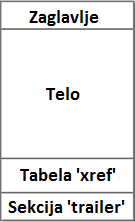
\includegraphics[width=0.2\textwidth]{pdfStruktura1.png}
\caption{Структура PDF датотека}
\label{fig:pdfStruktura1}
\end{figure}

\begin{description}
\item \textbf{Заглавље} Прва линија датотеке чини њено заглавље и садржи број PDF верзије која је коришћена у датотеци. У случају да се у датотеци налазе и бинарни подаци, потребно је у заглавље додати и другу линију која садржи најмање четири бинарна карактера (ASCII вредност им је већа или једнака од 128). Друга линија служи као индикатор да се у датотеци налазе бинарни подаци, што је корисно апликацијама које раде са PDF датотекама.
\item \textbf{Тело} Садржи све индиректне објекте који се налазе у датотеци.
Сви објекти су смештени у стабло, чији је корен каталог објекат (енг. \textit{document catalog}). Корен садржи информације о PDF датотеци и реферише на друге објекте који дефинишу податке датотеке. 

Подстабло (стабла свих објеката) које садржи све објекте страница се назива "\textit{стабло страница}" (енг. \textit{page tree}). 
\item \textbf{Табела "xref"} Табела "xref" или "\textit{cross reference}" табела садржи податке о свим објектима у датотеци и омогућава брз приступ било ком објекту датотеке. Уместо претраге целе датотеке у потрази за одређеним објектом, локација објекта се прочита из табеле након чега му се може директно приступити.

Сваки објекат описан је једним редом у табели дужине 20 бајтова. Првих 10 бајтова имају различиту намену у зависности од врсте објекта. Постоје две врсте објеката: \textit{валидни} и \textit{ослобођени} објекти. Ове две врсте објеката, као и само ослобађање су објашњени у поглављу \ref{sec:azuriranje}. 

У случају валидног објекта, првих 10 бајтова садржи локацију објекта у датотеци. Локација објекта је одређена помоћу удаљености (енг. \textit{offset}) почетка датотеке до почетка дефиниције објекта. У случају ослобођеног објекта, првих 10 бајтова садржи број следећег ослобођеног објекта (референцу на следећи ослобођени објекат у повезаној листи свих ослобођених објеката).

Након првих 10 бајтова, у случају обе врсте објекта следи \textit{генерацијски број} (енг. \textit{generation/revision number}), који се увећава сваки пут када се објекат ослободи. Након генерацијског броја налази се индикатор који говори о врсти објекта: 'f' за ослобођен објекат или 'n' за валидан објекат. 
\item \textbf{"Trailer"} Ова секција датотеке се дефинише кључном речју \textbf{trailer}. Овде се налази речник који садржи информације о датотеци као нпр. број редова у табели "xref", референца на каталог објекат, итд. Најважнија информација је информација о локацији "xref" табеле тј. о удаљености почетка датотеке до почетка дефиниције "xref" табеле. Број бајтова који представља удаљеност се наводи након кључне речи \textbf{startxref}. Локација "xref" табеле је важна јер омогућава брз приступ самој табели која даље својом структуром омогућава брз приступ објектима датотеке. Последња линија "trailer" секције садржи индикатор за крај датотеке "$\%\%EOF$".
\end{description}

\section{Ажурирање датотека}
\label{sec:azuriranje}


PDF датотеке се могу мењати, чиме се мења њихова структура тј. објекти у њима. Ажурирање датотеке не подразумева брисање или мењање постојећих података, већ додавање нових података на сам крај датотеке. Рецимо, заменом слике из датотеке новом сликом, објекат који представља стару слику неће бити обрисан или промењен тако да му садржај представља нову слику. Уместо тога, објекат старе слике биће означен као \textbf{ослобођен}, док ће објекат нове слике бити додат на сам крај датотеке. Тачније, ажурирањем датотеке се додаје ново тело, нова "xref" табела и нова "trailer" секција на крај датотеке. Ажурирање се може обављати неограничен број пута, при чему свака итерација (свако ажурирање) додаје три нове секције на крај датотеке. PDF датотека која је ажурирана $n$ пута је илустрована на слици \ref{fig:pdfStruktura2}. 

У новом телу се налазе нови или измењени објекти датотеке. Нова "xref" табела садржи искључиво локације нових, измењених и ослобођених објеката. Локације старих објеката се и даље читају из старе "xref" табеле ("xref" табеле претходне итерације). До старих објеката се лако долази, јер нова "trailer" секција поред локације нове "xref" табеле садржи и локацију претходне "xref" табеле. 

Сваки објекат који се обрише или измени постаје ослобођен, док се они који нису ослобођени називају \textbf{валидни} објекти. Сви ослобођени објекти се налазе у једној повезаној листи. Они се третирају као обрисани и не могу бити у садржају датотеке, а референце на њих су једнаке "Null" објекту. Ипак, објекат који је ослобођен може поново постати валидан неким наредним ажурирањем. \textit{Генерацијски број} објекта нам говори о укупном броју ослобађања једног објекта \cite{PDFDoc, introToPdf, basicStrPdf}.

Ажурирање датотеке на овај начин омогућава да се мале измене у великом документу брзо сачувају. Такође, некада је важно сачувати оригиналан садржај датотеке \cite{PDFDoc}.


\begin{figure}[t!]
\centering
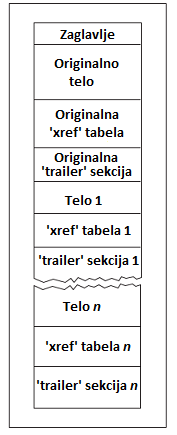
\includegraphics[width=0.3\textwidth]{pdfStruktura2.png}
\caption{Структура ажуриране PDF датотекe}
\label{fig:pdfStruktura2}
\end{figure}

% ------------------------------------------------------------------------------

% ------------------------------------------------------------------------------
\chapter{Закључак}
% ------------------------------------------------------------------------------

% ------------------------------------------------------------------------------
% Literatura
% ------------------------------------------------------------------------------
\literatura

% ==============================================================================
% Završni deo teze i prilozi
\backmatter
% ==============================================================================

% ------------------------------------------------------------------------------
% Biografija kandidata
\begin{biografija}
\textbf{Вук Стефановић Караџић} (\emph{Тршић, 26. октобар/6. новембар
  1787. — Беч, 7. фебруар 1864.}) био је српски филолог, реформатор
српског језика, сакупљач народних умотворина и писац првог речника
српског језика.  Вук је најзначајнија личност српске књижевности прве
половине XIX века. Стекао је и неколико почасних доктората.
Учествовао је у Првом српском устанку као писар и чиновник у
Неготинској крајини, а након слома устанка преселио се у Беч,
1813. године. Ту је упознао Јернеја Копитара, цензора словенских
књига, на чији је подстицај кренуо у прикупљање српских народних
песама, реформу ћирилице и борбу за увођење народног језика у српску
књижевност. Вуковим реформама у српски језик је уведен фонетски
правопис, а српски језик је потиснуо славеносрпски језик који је у то
време био језик образованих људи. Тако се као најважније године Вукове
реформе истичу 1818., 1836., 1839., 1847. и 1852.
\end{biografija}
% ------------------------------------------------------------------------------

\end{document} 